%!TeX root=MemoriaTFG.tex

\chapter{Metodologia d'Entrenament}
\label{cap:metodologia}

Aquest capítol descriu el procés experimental que ha portat des d'agents incapaços de
batre una heurística senzilla fins a un agent competitiu. L'enfocament és incremental:
cada fase planteja una hipòtesi concreta, dissenya un experiment per validar-la,
n'analitza els resultats i pren una decisió que condiciona la fase següent. Aquesta
estructura (\emph{hipòtesi $\rightarrow$ disseny $\rightarrow$ resultats $\rightarrow$
decisió}) permet aïllar l'efecte de cada tècnica i justificar per què el treball avança
en una direcció i no en una altra.

Les fases s'agrupen en tres blocs. Els dos primers es tanquen amb un punt de control
(\emph{checkpoint}) que fixa quins models continuen; el tercer culmina amb la decisió
del model de desplegament:

\begin{itemize}
  \item \textbf{Bloc 1} (secció~\ref{sec:bloc1}): línia base comparativa i
        \emph{curriculum learning} (Fases 1--2, Checkpoint~1).
  \item \textbf{Bloc 2} (secció~\ref{sec:bloc2}): representació de l'estat i memòria
        (Fases 3, 3.5 i 4, Checkpoint~2).
  \item \textbf{Bloc 3} (secció~\ref{sec:bloc3}): robustesa i aproximació a l'equilibri
        (Fases 5--6), amb la decisió final del model de desplegament.
\end{itemize}

\section{Marc metodològic comú}
\label{sec:marc-metodologic}

Totes les fases comparteixen el mateix protocol d'avaluació, la mateixa mètrica i el
mateix oponent de referència. Aquesta secció els defineix una vegada per no repetir-los
a cada fase.

\subsection*{Protocol d'avaluació}

El rendiment d'un agent es mesura amb la funció \texttt{evaluar\_agent()}, que juga un
nombre fix de partides senceres contra dos oponents de referència: 100~partides contra
un agent aleatori (\texttt{RandomAgent}) i 100~partides contra l'agent de regles
(\texttt{AgentRegles}). Per evitar el biaix posicional (ser \emph{mà} dona un lleuger
avantatge), l'agent alterna la seva posició (jugador~0 i jugador~1) en partides
consecutives. L'avaluació es fa cada 500\,000~passos d'entrenament i sempre sobre
\textbf{partides senceres}, encara que l'agent s'estigui entrenant sobre mans
individuals; així es mesura sempre la competència real al joc complet.

\subsection*{Mètrica de rendiment}

S'ha triat el \emph{win-rate} (percentatge de partides guanyades) com a base de la
mètrica, en lloc de la recompensa acumulada, per tres motius: és l'objectiu últim del joc,
és directament interpretable i és comparable entre algorismes diferents. Aquest darrer
punt és el més important. La recompensa d'entrenament de PPO i la de DQN no són
directament comparables perquè cada algorisme optimitza una quantitat interna distinta:
PPO maximitza un objectiu de gradient de política sobre l'avantatge estimada, mentre que
DQN minimitza l'error de diferència temporal de la seva funció~$Q$ (secció~\ref{sec:dqn} i
secció~\ref{sec:ppo}). A més, els dos algorismes usen factors de descompte diferents
($\gamma = 0{,}995$ per a PPO i $\gamma = 0{,}99$ per a DQN), de manera que ni tan sols el
retorn acumulat es mesura a la mateixa escala. El win-rate, en canvi, és una mètrica
\emph{externa}: es calcula jugant partides i comptant victòries, amb independència de com
s'ha entrenat l'agent, i per això permet comparar qualsevol parella d'algorismes en
igualtat de condicions. La mètrica combina el win-rate contra dos oponents complementaris:

\begin{equation}
  \text{metric} = 0{,}25 \cdot \text{wr}_{\text{random}} + 0{,}75 \cdot \text{wr}_{\text{regles}}
  \label{eq:metric}
\end{equation}

Cada terme compleix una funció diferent. L'\texttt{AgentRegles} (pes 0{,}75) és l'oponent
\textbf{discriminant}: batre una heurística coherent requereix estratègia real, de manera
que aquest terme és el que captura la qualitat de l'agent. El \texttt{RandomAgent}
(pes 0{,}25) actua com a \textbf{xarxa de seguretat}: guanyar-li és trivial, però un agent
que no hi guanyi de manera clara revela un col·lapse de la política (per exemple, una
política degenerada que repeteix sempre la mateixa acció). Aquest terme detecta
degeneracions que el win-rate contra regles, per si sol, podria emmascarar. El pes
dominant recau, doncs, sobre l'oponent que de debò discrimina l'habilitat, mentre que el
terme aleatori aporta un sòl d'estabilitat. Les fases avançades (5 i 6) introdueixen
mètriques addicionals de robustesa i explotabilitat, que es defineixen al bloc
corresponent.

\subsection*{L'oponent de referència: l'agent de regles}

L'\texttt{AgentRegles} (\texttt{RL/models/model\_propi/agent\_regles.py}) és un agent
heurístic codificat a mà que serveix alhora com a oponent d'entrenament i d'avaluació.
No té cap xarxa neuronal: la seva política prové d'heurístiques amb llindars adaptatius
sobre la força de la mà, els punts d'envit i el marcador.

\paragraph{La variant equilibrada i els seus paràmetres.} El comportament base de l'agent
(la variant \emph{equilibrada}) està governat per quatre paràmetres, cadascun amb un valor
neutre que es pren com a referència. Cada paràmetre modula un aspecte de la política:

\begin{itemize}
  \item \texttt{envit\_agressio} (neutre 1{,}0): escala els llindars de punts per acceptar
        o apujar l'envit. Amb el valor neutre, l'agent apuja l'envit a partir de
        30~punts de mà i l'accepta a partir de 25; el paràmetre divideix aquests
        llindars, de manera que un valor més alt els abaixa (accepta amb mans més febles)
        i un de més baix els apuja (més conservador). Els llindars també s'ajusten segons
        el marcador: si el rival és a punt de guanyar la partida, l'agent es torna
        conservador; si l'envit pot donar-li la partida, es torna agressiu.
  \item \texttt{truc\_agressio} (neutre 1{,}0): probabilitat d'apostar el truc en
        situacions favorables (per exemple, havent guanyat una ronda i amb una carta
        alta). Amb 1{,}0 aposta sempre en aquests casos; valors menors el fan dubtar i
        valors majors hi afegeixen farols addicionals.
  \item \texttt{farol\_prob} (neutre 0{,}12): probabilitat d'apostar el truc \emph{sense}
        una mà forta, és a dir, de fer farol.
  \item \texttt{resposta\_truc} (neutre 1{,}0): disposició a acceptar un truc cantat pel
        rival. Ajusta el llindar de força exigit per acceptar: valors superiors a~1
        accepten amb menys mà, valors inferiors es retiren més sovint.
\end{itemize}

\paragraph{Estocasticitat.} La característica clau de l'agent és que és
\textbf{estocàstic}: sobre les decisions deterministes anteriors hi injecta soroll
aleatori ($\pm2$ punts als llindars d'envit, $\pm5$ al llindar de força del truc, i
decisions probabilístiques a les zones grises de cada llindar). Aquesta estocasticitat és
deliberada i essencial. Un oponent purament determinista seria fàcilment explotable:
l'agent d'\ac{AR} aprendria a predir-ne les respostes fixes i el batria de manera
artificial, inflant la mètrica sense reflectir cap habilitat real (\emph{reward hacking}
contra un oponent fix). El soroll obliga l'agent entrenat a generalitzar i fa de
l'\texttt{AgentRegles} una barrera molt més exigent del que sembla.

\paragraph{El pool de variants.} A partir de la Fase~4, els quatre paràmetres es
modifiquen per generar sis \textbf{variants} amb estils de joc contrastats, que formen un
\emph{pool} d'oponents (taula~\ref{tab:pool-variants}): des de la conservadora (poc
agressiva i gairebé sense farol) fins a la farolera (màxima probabilitat de farol),
passant per especialistes en truc o en envit. La variant equilibrada hi figura amb els
valors neutres descrits més amunt.

\begin{table}[H]
  \centering
  \begin{tabular}{lcccc}
    \toprule
    Variant & \texttt{truc\_agressio} & \texttt{envit\_agressio} & \texttt{farol\_prob} & \texttt{resposta\_truc} \\
    \midrule
    Equilibrat  & 1{,}0 & 1{,}0 & 0{,}12 & 1{,}0 \\
    Conservador & 0{,}5 & 0{,}5 & 0{,}02 & 0{,}6 \\
    Agressiu    & 1{,}8 & 1{,}8 & 0{,}30 & 1{,}5 \\
    Truc-bot    & 2{,}0 & 0{,}4 & 0{,}15 & 1{,}2 \\
    Envit-bot   & 0{,}4 & 2{,}0 & 0{,}05 & 0{,}7 \\
    Faroler     & 1{,}3 & 1{,}3 & 0{,}40 & 1{,}3 \\
    \bottomrule
  \end{tabular}
  \caption{Les sis variants de l'\texttt{AgentRegles} que formen el \emph{pool}
           d'oponents (Fases 4--6). La variant equilibrada (primera fila) reprodueix el
           comportament per defecte usat a les fases 1--3.}
  \label{tab:pool-variants}
\end{table}

\subsection*{Convencions comunes}

Llevat que s'indiqui el contrari, tots els agents comparteixen l'arquitectura base de
xarxa (\ac{MLP} de dues capes ocultes de 256~unitats amb ReLU) i s'avaluen sobre
l'observació de 240~dimensions descrita al capítol~\ref{cap:entorns}. El pressupost
d'entrenament s'expressa en \emph{timesteps} (passos d'interacció amb l'entorn). Els
hiperparàmetres complets de cada algorisme i fase es recullen a
l'annex~\ref{ann:hiperparametres}; al cos del capítol només se'n destaquen els rellevants
per a cada decisió.

%!TeX root=MemoriaTFG.tex

\section{Bloc 1: línia base i \emph{curriculum learning}}
\label{sec:bloc1}

El primer bloc estableix un punt de partida rigorós (Fase~1) i introdueix la primera
tècnica que trenca el sostre de rendiment inicial (Fase~2, \emph{curriculum learning}).
El Checkpoint~1 tanca el bloc seleccionant els dos models que continuen.

\subsection{Fase 1: comparativa homogènia d'algorismes}
\label{sec:fase1}

\paragraph{Hipòtesi.} Abans d'aplicar cap tècnica avançada cal saber quin algorisme
parteix amb avantatge. La Fase~1 compara quatre algorismes d'\ac{AR} en igualtat de
condicions i partint de zero, sense cap coneixement previ del joc.

\paragraph{Disseny.} Es comparen quatre agents que cobreixen les dues grans famílies
d'algorismes d'\ac{AR}: els \textbf{basats en la funció de valor} (com el DQN, que aprèn
quant val cada acció i n'extreu la política) i els \textbf{basats en el gradient de la
política} (com el PPO, que optimitza directament la política). Es reparteixen també entre
les variants \emph{on-policy} i \emph{off-policy} (definides al capítol~\ref{cap:marc}) i
entre les dues biblioteques emprades (taula~\ref{tab:fase1-algorismes}). Tots comparteixen
la mateixa observació de
240~dimensions, la mateixa arquitectura \ac{MLP} de \([256, 256]\) sense extractor
convolucional, i la mateixa funció d'avaluació; així qualsevol diferència s'atribueix a
l'algorisme i no a l'arquitectura.

\begin{table}[H]
  \centering
  \begin{tabular}{llll}
    \toprule
    Algorisme & Biblioteca & Política & Paral·lelisme \\
    \midrule
    DQN-RLCard  & RLCard & Off-policy        & 1 entorn seqüencial \\
    NFSP-RLCard & RLCard & Off-policy + \acs{SL} & 1 entorn seqüencial \\
    DQN-SB3     & \ac{SB3} & Off-policy      & 1 entorn \\
    PPO-SB3     & \ac{SB3} & On-policy       & 48 entorns (\emph{SubprocVecEnv}) \\
    \bottomrule
  \end{tabular}
  \caption{Els quatre algorismes comparats a la Fase~1.}
  \label{tab:fase1-algorismes}
\end{table}

\emph{Avaluació en dues òptiques.} Com que els algorismes tenen velocitats molt
diferents, comparar-los només per passos seria injust amb els paral·lelitzables. Per això
es mesura el rendiment sota dues òptiques complementàries:
\begin{itemize}
  \item \textbf{Per passos} (5~milions): la qualitat assolida després del mateix nombre de
        passos d'entrenament (eficiència per mostra).
  \item \textbf{Per temps real} (4~hores per agent): la qualitat assolida amb el mateix
        pressupost temporal (rendiment efectiu segons el \emph{throughput}).
\end{itemize}

\emph{Oponents.} Cada agent s'entrena contra una barreja d'oponents
(taula~\ref{tab:fase1-oponents}) amb un criteri comú: una petita fracció de
l'agent aleatori (per mantenir diversitat i explorar estats poc habituals) i un gruix
de l'agent basat en regles (el senyal estratègic principal). La diferència és el
\emph{self-play}: els agents de RLCard (DQN i NFSP) el suporten de manera nativa, de manera
que un 30\% de les partides es juguen contra una versió del propi agent. En el cas del DQN,
aquesta versió és una còpia \emph{Polyak} que s'actualitza lentament (un 5\% cap als pesos  
actuals cada 5\,000~passos): així l'oponent millora amb l'agent però no canvia tan de
pressa com per desestabilitzar l'aprenentatge.

\begin{table}[H]
  \centering
  \begin{tabular}{lccc}
    \toprule
    Agent & Random & l'agent basat en regles & Self-play \\
    \midrule
    DQN-RLCard  & 10\%      & 60\%       & 30\% (Polyak) \\
    NFSP-RLCard & 10\%      & 60\%       & 30\% (natiu) \\
    DQN-SB3     & 5\%       & 95\%       & — \\
    PPO-SB3     & 5\%       & 95\%       & — \\
    \bottomrule
  \end{tabular}
  \caption{Distribució d'oponents per episodi a la Fase~1. Els agents de RLCard
           incorporen self-play; els de \ac{SB3} entrenen només contra oponents fixos
           (l'agent aleatori i l'agent basat en regles), sense self-play.}
  \label{tab:fase1-oponents}
\end{table}

\emph{Bucle d'entrenament.} Els dos agents de RLCard s'entrenen
amb un bucle manual: controla el
format de cada transició que s'injecta al \emph{replay buffer}, alterna la posició de
l'aprenent a cada partida i resol l'assignació de crèdit quan és l'oponent qui tanca la
partida (la recompensa terminal s'assigna a la darrera jugada de l'aprenent). Els agents
\ac{SB3} usen la rutina nativa de la biblioteca amb un \emph{callback} que avalua i desa el
millor model cada 500\,000~passos. PPO genera l'experiència amb 48~entorns en paral·lel
repartits entre oponents i posicions. Per garantir que l'avaluació mesura generalització i
no memorització, l'agent basat en regles de l'avaluació s'instancia amb una llavor diferent
de la d'entrenament.

\paragraph{Resultats.} Cap agent assoleix un rendiment alt \emph{i} estable alhora
(taula~\ref{tab:fase1-resultats}). DQN-SB3 és el millor en totes dues òptiques (pic del
62{,}8\% per passos i 58{,}5\% per temps), però pateix una degradació severa cap al final
de l'entrenament (de 62{,}8\% a 36{,}5\%): la seva millor mètrica és molt superior a la
final. PPO-SB3 és el més feble a igualtat de passos (29{,}5\%), perquè un algorisme
on-policy necessita molts més passos per estabilitzar-se, però té un \emph{throughput}
incomparable (taula~\ref{tab:fase1-throughput}): genera 36{,}5~milions de passos per hora,
28~vegades més que NFSP. Aquest contrast fa que el rànquing canviï entre les dues òptiques.
El patró comú a tots els agents és la \textbf{inestabilitat}: regredeixen cap al final de
l'entrenament, senyal que el problema (partida llarga, recompensa molt diferida) no
proporciona un senyal d'aprenentatge prou estable.

\begin{table}[H]
  \centering
  \begin{tabular}{lcccc}
    \toprule
    & \multicolumn{2}{c}{Per passos (5M)} & \multicolumn{2}{c}{Per temps (4~h)} \\
    \cmidrule(lr){2-3}\cmidrule(lr){4-5}
    Agent & Millor & Final & Millor & Final \\
    \midrule
    DQN-SB3     & \textbf{62{,}8\%} & 36{,}5\% & \textbf{58{,}5\%} & 17{,}2\% \\
    NFSP-RLCard & 53{,}2\% & 29{,}0\% & 43{,}0\% & 33{,}2\% \\
    DQN-RLCard  & 51{,}0\% & 25{,}8\% & 44{,}5\% & 34{,}2\% \\
    PPO-SB3     & 29{,}5\% & 18{,}5\% & 42{,}0\% & 21{,}2\% \\
    \bottomrule
  \end{tabular}
  \caption{\texttt{metric} de la Fase~1 sota les dues òptiques. «Millor» és el pic durant
           l'entrenament; «Final» és el valor en acabar, que evidencia la inestabilitat.}
  \label{tab:fase1-resultats}
\end{table}

\begin{table}[H]
  \centering
  \begin{tabular}{lrr}
    \toprule
    Algorisme & Passos/hora & Factor vs NFSP \\
    \midrule
    PPO-SB3     & 36{,}5\,M & 28$\times$ \\
    DQN-SB3     & 7{,}0\,M  & 5{,}4$\times$ \\
    DQN-RLCard  & 5{,}5\,M  & 4{,}2$\times$ \\
    NFSP-RLCard & 1{,}3\,M  & 1$\times$ \\
    \bottomrule
  \end{tabular}
  \caption{\emph{Throughput} dels quatre algorismes. El paral·lelisme de PPO-SB3 el fa
           28~vegades més ràpid que NFSP-RLCard.}
  \label{tab:fase1-throughput}
\end{table}

\begin{figure}[H]
  \centering
  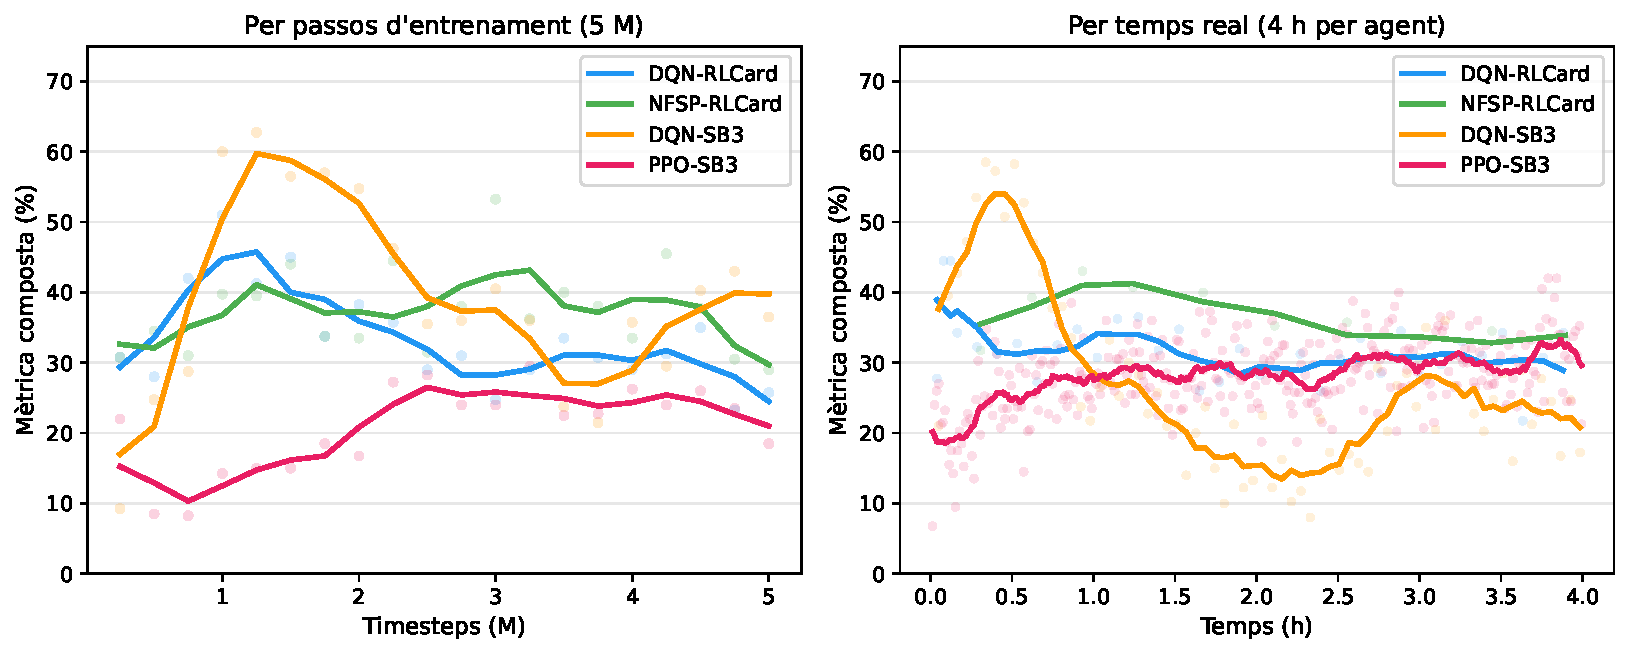
\includegraphics[width=\textwidth]{figures/fase1/corbes_ts.pdf}
  \caption{Mètrica composta de la Fase~1 sota les dues òptiques d'avaluació.
           A l'esquerra, rendiment als 5~M passos d'entrenament (eficiència per
           mostra); a la dreta, rendiment al llarg de 4~hores de còmput per agent
           (rendiment efectiu). DQN-SB3 lidera en ambdues, però el rànquing
           de la resta canvia: PPO-SB3 és el pitjor per passos però supera
           DQN-RLCard i NFSP-RLCard per temps gràcies al seu \emph{throughput}.}
  \label{fig:fase1-corbes-ts}
\end{figure}

\paragraph{Decisió.} El coll d'ampolla no és el còmput sinó el \textbf{senyal
d'aprenentatge}. El cas més clar és PPO-SB3: és l'agent més escalable i ràpid, però el que
menys aprofita una partida llarga amb recompensa diferida. La hipòtesi que en sorgeix és
que factoritzar la partida en unitats més curtes i denses (mans) hauria de donar un senyal
molt més ric. Això motiva la Fase~2.

\emph{Nota sobre l'observació.} Les Fases~1 i~2 van utilitzar una versió primerenca del
vector de context de 23~dimensions (239~dimensions en total). A partir de la Fase~3 es va
ampliar a 24~dimensions (240 en total), tal com es descriu al capítol~\ref{cap:entorns}.
El canvi no afecta les conclusions comparatives, atès que totes les sèries d'una mateixa
fase comparteixen la mateixa observació.

\subsection{Fase 2: \emph{curriculum learning} (mà $\rightarrow$ partida)}
\label{sec:fase2}

\paragraph{Hipòtesi.} Entrenar directament sobre partides senceres obliga l'agent a
resoldre alhora dos problemes acoblats: jugar bé cada mà (tàctica local) i gestionar el
marcador al llarg de la partida (estratègia global). El \emph{curriculum
learning}~\cite{bengio2009curriculum}, que presenta primer els exemples simples i després
els complexos, permet desacoblar-los. Al Truc, una \emph{mà} és la unitat natural simple:
episodi curt ($\sim$15~passos) i recompensa calculable al final. La hipòtesi és que
entrenar primer sobre mans (amb l'entorn \texttt{TrucEnvMa} descrit al
capítol~\ref{cap:entorns}) i després fer \emph{finetune} sobre partides senceres accelera i
millora l'aprenentatge respecte a entrenar-hi directament.

\paragraph{Disseny.}

\emph{El curriculum de dues etapes.} S'ha dissenyat un curriculum que va de la tasca densa
i curta a l'escassa i llarga (figura~\ref{fig:fase2-curriculum}):
\begin{enumerate}
  \item \textbf{Etapa de mans} (12M passos): l'agent s'entrena a \texttt{TrucEnvMa}, on
        cada mà és un episodi independent ($\sim$15~passos) amb recompensa densa
        normalitzada ($\text{punts}/24$). Aquí aprèn la tàctica local: quan jugar fort,
        quan acceptar un envit, quan plantar el truc.
  \item \textbf{Etapa de partides} (12M passos): els pesos apresos es transfereixen a
        \texttt{TrucEnv}, on l'episodi és una partida sencera fins a 24~punts. L'agent
        parteix d'una política ja formada i el \emph{finetune} recau sobre l'estratègia a
        llarg termini, com la gestió del marcador.
\end{enumerate}

\begin{figure}[H]
  \centering
  \begin{tikzpicture}[
      box/.style={draw, rounded corners=3pt, minimum width=3.6cm, minimum height=1.5cm,
                  align=center, font=\small},
      arr/.style={-{Stealth}, thick}
  ]
    \node[box] (mans) {\textbf{Etapa 1: Mans}\\12M passos\\recompensa densa};
    \node[box, right=2.8cm of mans] (partides) {\textbf{Etapa 2: Partides}\\12M passos\\recompensa escassa};
    \draw[arr] (mans) -- node[above, font=\footnotesize]{transferència $\theta$} (partides);
  \end{tikzpicture}
  \caption{Currículum de dues etapes: mans individuals amb recompensa densa, seguides de
           partides senceres amb transferència dels pesos apresos ($\theta$).}
  \label{fig:fase2-curriculum}
\end{figure}

\emph{Comparació experimental.} Per a cada algorisme s'executen dues configuracions amb el
mateix pressupost total de 24~milions de passos: \textbf{control} (24M directament sobre
partides) i \textbf{curriculum} (les dues etapes anteriors). Per aïllar l'efecte del
curriculum s'elimina el \emph{self-play} i tots els agents s'entrenen amb la mateixa
distribució d'oponents (10\% Random + 90\% Regles). L'avaluació es fa sempre sobre partides
senceres, encara que l'agent estigui aprenent sobre mans, perquè és on es vol mesurar la
competència real.

\emph{Transferència al finetune.} El pas de l'etapa de mans a la de partides no és
automàtic: els pesos de la primera etapa (\texttt{best\_mans}) es carreguen explícitament
abans de la segona, via \texttt{PPO.load()} o carregant l'estat de la xarxa~$Q$ segons
l'agent. A més, per al DQN-SB3 es redueix l'exploració inicial del \emph{finetune}
($\varepsilon = 0{,}10$ en lloc d'1{,}0) i s'escurça el \emph{warmup}, perquè la política ja
està formada i no cal tornar a explorar des de zero.

\emph{Riscos.} El principal és l'\textbf{oblit catastròfic}: els algorismes on-policy com
PPO descarten les dades antigues a cada actualització, de manera que l'agent podria oblidar
el que va aprendre sobre mans en exposar-se a les partides. Un segon risc és el desajust de
distribució, ja que la distribució de mans amb el marcador a 0--0 difereix de la que
apareix amb el marcador avançat.

\paragraph{Resultats.} La taula~\ref{tab:fase2-12m} mostra que, a igualtat de pressupost
(12M passos), entrenar sobre mans és \emph{uniformement} superior a entrenar sobre
partides per als quatre agents, amb diferències espectaculars per als agents \ac{SB3}
(+42 i +56~punts percentuals). Aquesta és la validació clau: l'entorn per mans aporta un
senyal d'aprenentatge qualitativament millor. Ara bé, la taula~\ref{tab:fase2-24m} mostra
que la transferència d'aquest aprenentatge a partides senceres (després del \emph{finetune})
no és universal: només 2~de 4 agents en surten beneficiats al pressupost total. El coll
d'ampolla passa a ser la transferència, no l'aprenentatge inicial.

\begin{table}[H]
  \centering
  \begin{tabular}{lrrr}
    \toprule
    Agent & Control 12M & Curriculum 12M (mans) & $\Delta$ \\
    \midrule
    DQN-RLCard  & 18{,}2\% & 26{,}0\% & $+7{,}8$ \\
    NFSP-RLCard & 25{,}2\% & 27{,}2\% & $+2{,}0$ \\
    DQN-SB3     & 44{,}0\% & 86{,}2\% & $+42{,}2$ \\
    PPO-SB3     & 30{,}8\% & 87{,}2\% & $+56{,}5$ \\
    \bottomrule
  \end{tabular}
  \caption{Comparació a 12M passos (mateix pressupost, avaluació sobre partides). El
           valor \texttt{metric} entrenant sobre mans és uniformement superior.}
  \label{tab:fase2-12m}
\end{table}

\begin{table}[H]
  \centering
  \begin{tabular}{lrrr}
    \toprule
    Agent & Control 24M & Curriculum (12M+12M) & $\Delta$ \\
    \midrule
    DQN-RLCard  & 52{,}0\% & 22{,}2\% & $-29{,}8$ \\
    NFSP-RLCard & 55{,}5\% & 60{,}0\% & $+4{,}5$ \\
    DQN-SB3     & 60{,}5\% & 56{,}0\% & $-4{,}5$ \\
    PPO-SB3     & 35{,}0\% & 75{,}0\% & $+40{,}0$ \\
    \bottomrule
  \end{tabular}
  \caption{Comparació a 24M passos totals (control sencer vs curriculum complet). Només
           PPO-SB3 i NFSP-RLCard milloren; DQN-RLCard col·lapsa per oblit catastròfic.}
  \label{tab:fase2-24m}
\end{table}

\begin{figure}[H]
  \centering
  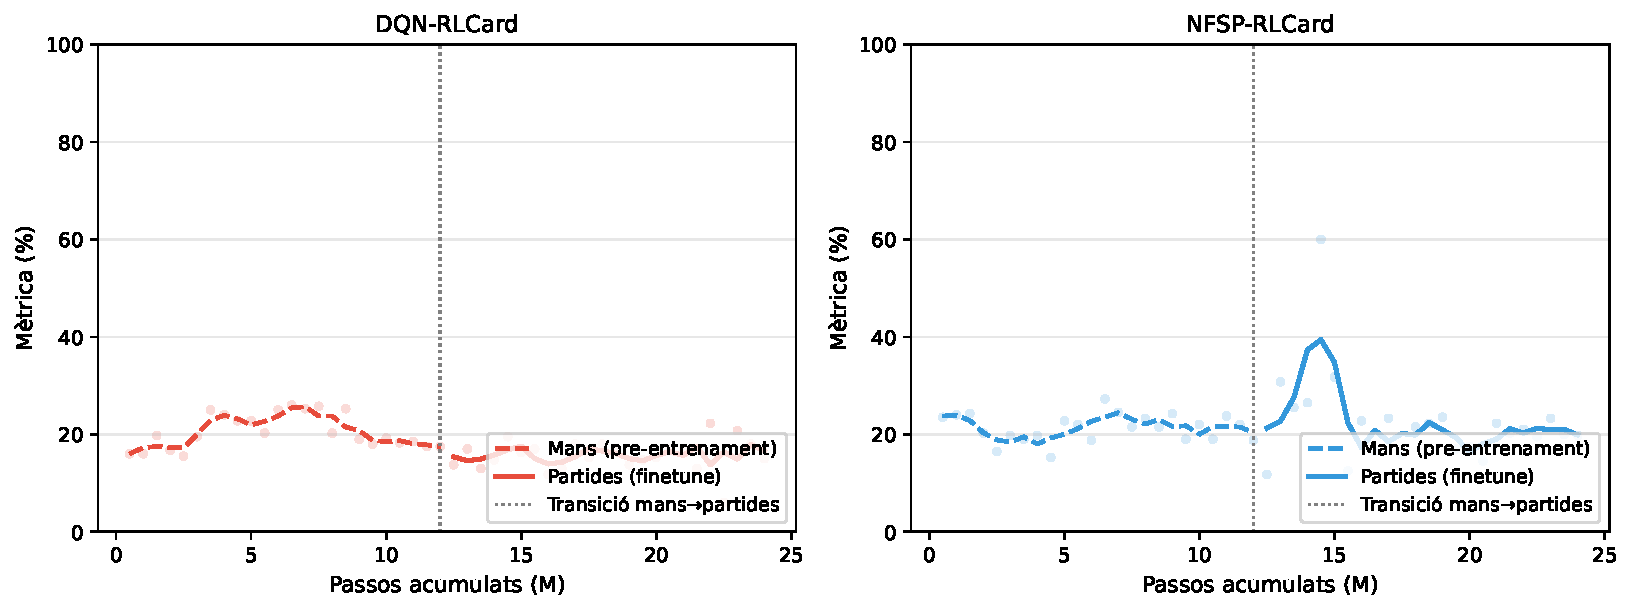
\includegraphics[width=\textwidth]{figures/fase2/curriculum_rlcard.pdf}
  \caption{Corbes del \emph{curriculum} per als agents RLCard. La línia ratllada
           és la fase de mans (pre-entrenament); la línia sòlida el \emph{finetune}
           sobre partides. La línia puntejada marca la transició als 12M passos.
           DQN-RLCard col·lapsa al \emph{finetune}; NFSP-RLCard recupera i millora
           lleugerament.}
  \label{fig:fase2-curriculum-rlcard}
\end{figure}

\begin{figure}[H]
  \centering
  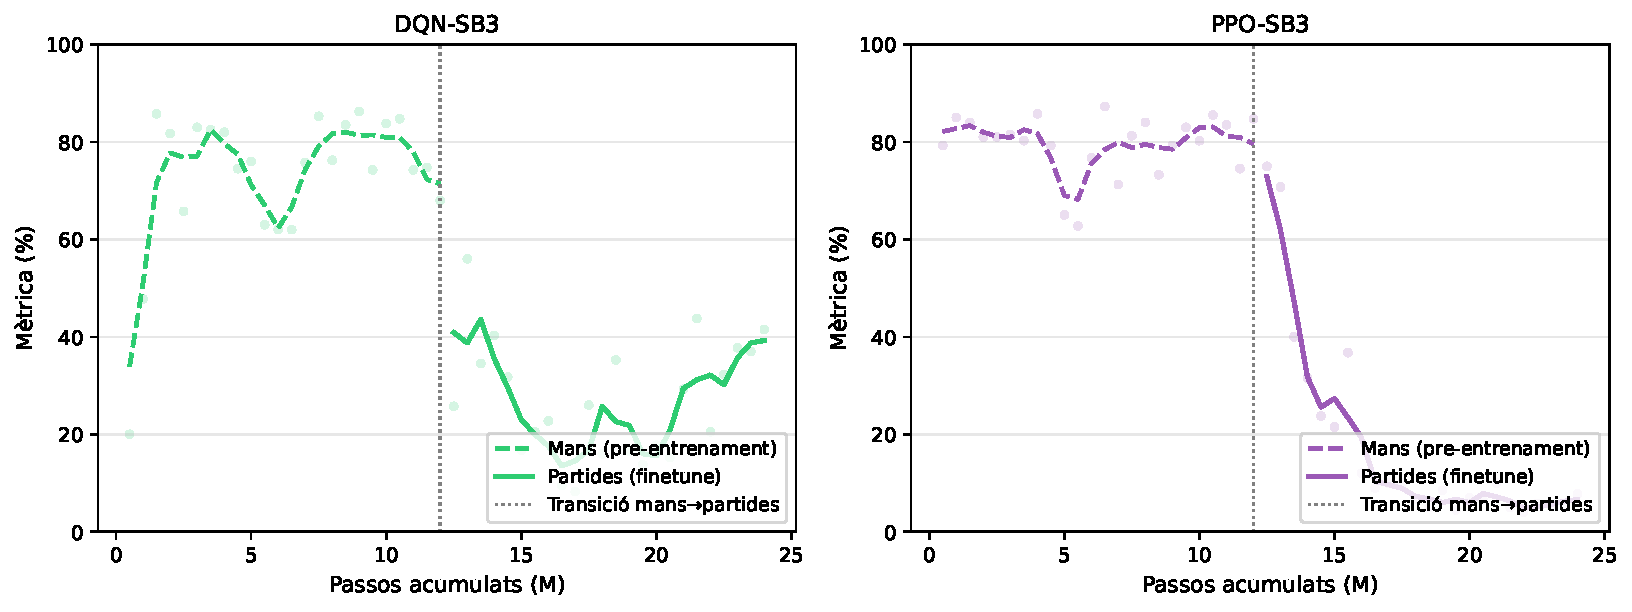
\includegraphics[width=\textwidth]{figures/fase2/curriculum_sb3.pdf}
  \caption{Corbes del \emph{curriculum} per als agents SB3. DQN-SB3 assoleix un pic
           alt en mans (86\%) però perd rendiment al \emph{finetune}. PPO-SB3 manté
           el nivell i tanca a 75\%, el millor resultat del treball fins al moment.}
  \label{fig:fase2-curriculum-sb3}
\end{figure}

El cas més destacat és \textbf{PPO-SB3}, l'agent més feble de la Fase~1: passa del 35\%
al 75\% amb el curriculum complet (+40~punts), el millor resultat del treball fins
aleshores. Es valida que el problema de PPO no era l'algorisme sinó l'horitzó llarg amb
recompensa diferida. En canvi, \textbf{DQN-RLCard} col·lapsa al \emph{finetune} (22{,}2\%):
la seva implementació no integra bé la càrrega de pesos previs i, sense el \emph{self-play}
regularitzador de la Fase~1, perd estabilitat.

\paragraph{Decisió.} El \emph{curriculum learning} millora el rendiment, però de manera
condicionada a l'agent: a igualtat de 12M passos tots quatre agents aprenen molt millor
sobre mans, però després del \emph{finetune} només PPO-SB3 (massivament) i NFSP-RLCard
(lleugerament) en surten beneficiats al pressupost total. El coll d'ampolla, doncs, és la
\textbf{transferència} de mans a partides, no l'aprenentatge inicial; i el curriculum
queda validat com a tècnica clau per a PPO-SB3.

\subsection{Checkpoint 1: models seleccionats}
\label{sec:checkpoint1}

Tancades les Fases~1 i~2, cal decidir quins dels quatre models continuen a la resta del
treball. El criteri combina el rendiment (\texttt{metric}) i el cost d'entrenament, i el
resultat és clar: avancen els dos agents \ac{SB3} i es descarten els dos de RLCard.

\textbf{PPO-SB3} és el gran beneficiari del curriculum i passa a ser el \emph{baseline} de
referència. Del 35\% puja al 75\% amb el curriculum complet (el millor resultat del treball
fins aleshores) i és el millor aprenent sobre mans (87,2\%), amb aproximadament la meitat
del cost de DQN-SB3 ($\sim$40~min davant de $\sim$5,5~h per execució). La seva narrativa
resumeix la lliçó del bloc: PPO no tenia un problema de capacitat sinó de senyal
d'aprenentatge, i el curriculum el resol. El seu \emph{throughput} excel·lent permet, a
més, iterar ràpidament a les fases següents. \textbf{DQN-SB3} es manté com a \emph{baseline}
robust: és el millor sobre partides sense curriculum (60,5\%), té un sostre del 86,2\% sobre
mans i representa la família dels algorismes basats en la funció de valor, el contrapunt
natural a PPO; el
seu cost ($\sim$5,5~h per execució) és assumible per als experiments llargs de les fases
següents.

Es descarten, en canvi, els dos agents de RLCard. \textbf{DQN-RLCard} pateix un oblit
catastròfic sever al \emph{finetune} (col·lapsa al 22\%) i és consistentment inferior a
DQN-SB3 en tots els experiments. \textbf{NFSP-RLCard} és l'algorisme més lent
($\sim$17~h per execució), no supera el 60\% de \texttt{metric} i no mostra cap
escalabilitat amb més còmput: el benefici és massa modest per al cost.

%!TeX root=MemoriaTFG.tex

\section{Bloc 2: representació de l'estat i memòria}
\label{sec:bloc2}

Amb els dos agents \ac{SB3} seleccionats al Checkpoint~1, el segon bloc explora dues
direccions ortogonals per superar el sostre de rendiment: millorar la \emph{representació}
de l'estat (Fase~3, dividida en arquitectura i inicialització del cos) i dotar l'agent de
\emph{memòria} entre mans (Fase~4). El Checkpoint~2 tanca el bloc fixant el model que
s'adopta per a desplegament.

\subsection{Fase 3: el feature extractor COS}
\label{sec:fase3}

\begin{sloppypar}
La Fase~3 estudia \texttt{CosMultiInput}, un \emph{feature extractor} convolucional
propi, com a alternativa a l'extractor pla per defecte de \ac{SB3}.
L'estudi respon dues preguntes acoblades: si l'\textbf{arquitectura} convolucional
aporta valor per si sola (Q1, secció~\ref{sec:fase3-arq}) i si
\textbf{inicialitzar-la} amb coneixement previ del joc desbloqueja un rendiment
superior (Q2, secció~\ref{sec:fase3-init}).
\end{sloppypar}

\subsubsection{Arquitectura: CNN vs MLP}
\label{sec:fase3-arq}

\paragraph{Hipòtesi.} El vector pla de 240~dimensions amaga l'estructura espacial del
tensor de cartes. Un \ac{MLP} pla ha de \emph{redescobrir} per ell mateix que el 4~de
Copes i el 4~d'Ors comparteixen rang, o que cartes de pals diferents poden tenir forces
relacionades. La hipòtesi (Q1) és que un extractor que respecta l'estructura
\(6 \times 4 \times 9\) del tensor de cartes (mitjançant convolucions) supera el \ac{MLP}
estàndard.

\paragraph{Disseny.}

\emph{L'extractor CosMultiInput.} Per provar la hipòtesi es
dissenya \texttt{CosMultiInput} (\texttt{RL/models/core/feature\_extractor.py}), un
extractor de dues branques (figura~\ref{fig:cos-multi-input}). La branca \acf{CNN} aplica
dues convolucions sobre el tensor \((6,4,9)\) (taula~\ref{tab:canals-cartes}): la primera amb nucli \(1\times3\) detecta
patrons entre rangs consecutius; la segona amb nucli \(3\times3\) integra la informació
entre pals i rangs, produint 320~dimensions. La branca densa projecta el vector de context
de 24~dimensions (taula~\ref{tab:context-obs}) a~32. Les dues sortides es concatenen i es projecten a 256~dimensions. La
sortida coincideix amb l'amplada de la primera capa oculta de la política
(\texttt{net\_arch=[256,256]}), de manera que \texttt{CosMultiInput} substitueix
l'extractor per defecte de \ac{SB3} (\texttt{CombinedExtractor}, que simplement aplana
l'observació) sense cap altre canvi. L'adaptador \texttt{CosMultiInputSB3} (\texttt{RL/%
\allowbreak{}models/\allowbreak{}sb3/\allowbreak{}sb3\_\allowbreak{}features\_%
\allowbreak{}extractor.py}) fa de pont entre el vector pla i les dues branques.

\begin{figure}[H]
  \centering
  \resizebox{\textwidth}{!}{%
  \begin{tikzpicture}[
      inp/.style ={draw, rounded corners=3pt, minimum width=2.2cm, minimum height=0.85cm,
                   align=center, font=\small, fill=blue!6},
      cnn/.style ={draw, rounded corners=3pt, minimum width=2.5cm, minimum height=0.75cm,
                   align=center, font=\footnotesize, fill=orange!10},
      ctx/.style ={draw, rounded corners=3pt, minimum width=2.5cm, minimum height=0.75cm,
                   align=center, font=\footnotesize, fill=teal!10},
      fus/.style ={draw, rounded corners=3pt, minimum width=2.5cm, minimum height=0.75cm,
                   align=center, font=\footnotesize, fill=purple!8},
      res/.style ={draw, rounded corners=3pt, minimum width=2.2cm, minimum height=0.85cm,
                   align=center, font=\small, fill=blue!6},
      arr/.style ={-{Stealth}, thick},
  ]
    % ── Branca CNN (fila superior) ─────────────────────────────────────────
    \node[inp] (cartes) {Tensor cartes\\$(6,4,9)$};
    \node[cnn, right=0.8cm of cartes]  (cnn1) {\texttt{Conv2d}\\$6{\to}16$, $1{\times}3$};
    \node[cnn, right=0.7cm of cnn1]   (cnn2) {\texttt{Conv2d}\\$16{\to}32$, $3{\times}3$};
    \node[cnn, right=0.7cm of cnn2]   (flat) {Flatten\\${\to}\,320$};

    % ── Branca context (fila inferior) ────────────────────────────────────
    \node[inp, below=1.6cm of cartes] (context) {Vector context\\$(24,)$};
    \node[ctx, right=0.8cm of context] (lin) {\texttt{Linear}\\$24{\to}32$};

    % ── Fusió ──────────────────────────────────────────────────────────────
    \node[fus, right=1.2cm of flat |- context, yshift=0.8cm]
          (cat)   {cat$([320,\,32])$\\$=352$};
    \node[fus, right=0.7cm of cat]  (fusio) {\texttt{Linear}\\$352{\to}256$};
    \node[res, right=0.7cm of fusio] (latent) {Latent\\$(256,)$};

    % ── Fletxes CNN ────────────────────────────────────────────────────────
    \draw[arr] (cartes)  -- (cnn1);
    \draw[arr] (cnn1)    -- (cnn2);
    \draw[arr] (cnn2)    -- (flat);
    \draw[arr] (flat)    -- (cat);

    % ── Fletxes context ────────────────────────────────────────────────────
    \draw[arr] (context) -- (lin);
    \draw[arr] (lin)     -| (cat);

    % ── Fletxes fusió ──────────────────────────────────────────────────────
    \draw[arr] (cat)   -- (fusio);
    \draw[arr] (fusio) -- (latent);
  \end{tikzpicture}%
  }
  \caption{\texttt{CosMultiInput}: arquitectura de dues branques. La branca CNN processa
           el tensor de cartes $(6,4,9)$; la branca lineal el vector de context $(24,)$.
           Les sortides es concatenen i es projecten a un vector latent de 256~dimensions.}
  \label{fig:cos-multi-input}
\end{figure}

\emph{Els tres protocols.} La comparació es fa sobre els tres protocols d'entrenament
introduïts a la Fase~2 (secció~\ref{sec:fase2}), que es recorden aquí perquè ara es
comparen tots tres:
\begin{itemize}
  \item \textbf{Control}: entrenar directament sobre \emph{partides senceres}; la condició
        de referència, sense cap facilitació.
  \item \textbf{Curriculum}: entrenar primer sobre \emph{mans} i després fer \emph{finetune}
        sobre partides senceres (el currículum de dues etapes de la Fase~2).
  \item \textbf{Mans}: entrenar \emph{exclusivament} sobre mans individuals, sense el pas
        posterior a partides.
\end{itemize}

\emph{Comparació experimental.} Per a cada protocol i agent es compara la variant COS (amb
pesos aleatoris) amb la variant \ac{MLP}, amb 24~milions de passos cada combinació i la
mateixa distribució d'oponents que la Fase~2 (10\% Random + 90\% Regles). Això suposa sis
runs nous amb COS i dos amb \ac{MLP} sobre mans; les quatre sèries \ac{MLP} de control i
curriculum es reutilitzen de la Fase~2 per no reentrenar-les.

\paragraph{Resultats.} El COS amb pesos aleatoris no supera sistemàticament el \ac{MLP}
(taula~\ref{tab:fase3}). Només aporta una millora clara al protocol de control per a
DQN-SB3 (+10{,}5~punts). El protocol \textbf{mans} torna a ser el millor en termes
absoluts (totes les combinacions superen el 82\%), però la diferència entre COS i \ac{MLP}
hi és marginal (\(<4\) punts). La inducció estructural per si sola, amb pesos aleatoris,
no és suficient per desbloquejar un avantatge. La lectura és coherent: al protocol de
control, sense cap facilitació, la capacitat addicional de la \ac{CNN} per extreure
patrons de l'estructura de les cartes es tradueix en un guany real; al protocol de mans,
el currículum d'entrenament sobre mans individuals ja exposa l'agent als patrons
carta-a-carta en un context simplificat, de manera que el \ac{MLP} arriba al protocol
de mans amb una representació prou rica i la \ac{CNN} no hi aporta res addicional.

\begin{table}[H]
  \centering
  \begin{tabular}{llrrr}
    \toprule
    Protocol & Agent & COS & \ac{MLP} & $\Delta$ \\
    \midrule
    Control    & DQN-SB3 & 71{,}0\% & 60{,}5\% & $+10{,}5$ \\
    Control    & PPO-SB3 & 32{,}5\% & 35{,}0\% & $-2{,}5$ \\
    Curriculum & DQN-SB3 & 56{,}2\% & 56{,}0\% & $+0{,}2$ \\
    Curriculum & PPO-SB3 & 63{,}0\% & 75{,}0\% & $-12{,}0$ \\
    Mans       & DQN-SB3 & 82{,}2\% & 85{,}8\% & $-3{,}6$ \\
    Mans       & PPO-SB3 & 89{,}0\% & 87{,}2\% & $+1{,}8$ \\
    \bottomrule
  \end{tabular}
  \caption{Pic de \texttt{metric} (24M passos) per a COS amb pesos aleatoris vs \ac{MLP}.}
  \label{tab:fase3}
\end{table}

\begin{figure}[H]
  \centering
  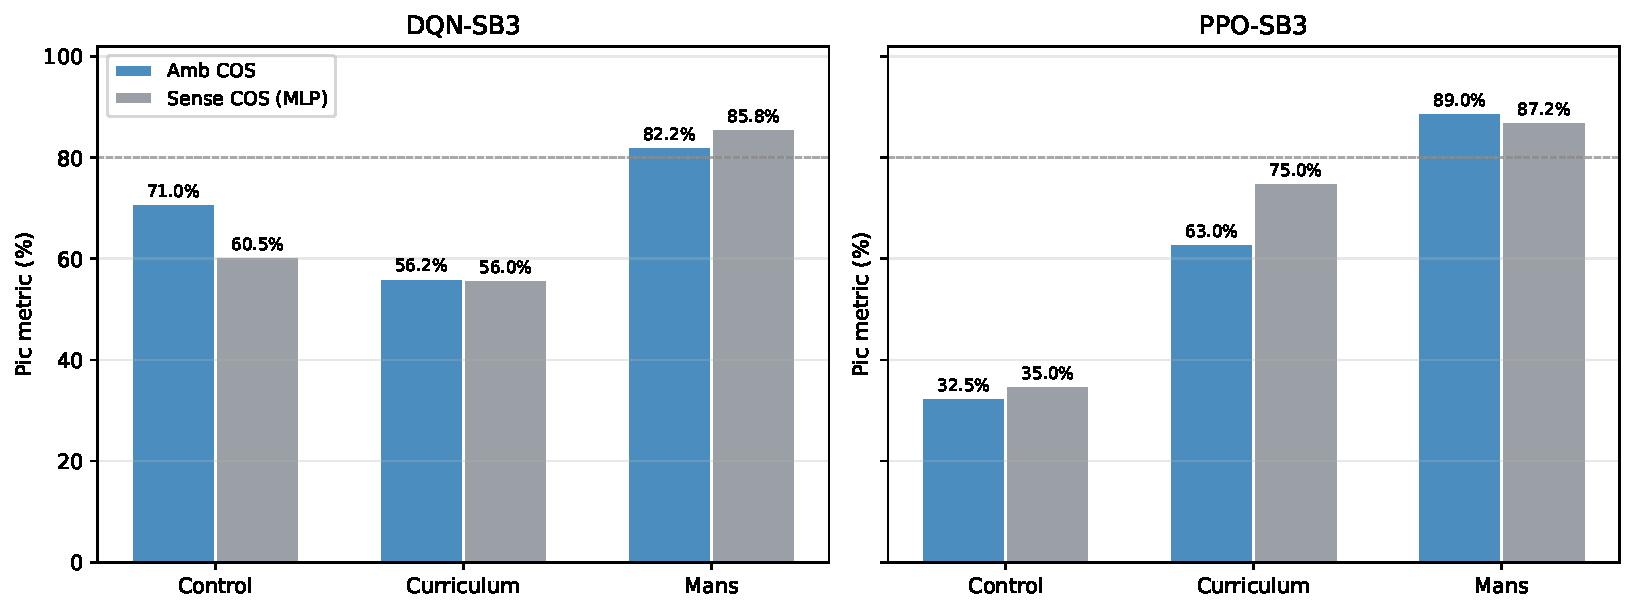
\includegraphics[width=\textwidth]{figures/fase3/fase3_cos_vs_mlp.pdf}
  \caption{Pic de \texttt{metric} (24M passos) per protocol i agent, COS amb pesos
           aleatoris vs \ac{MLP}. La línia discontínua marca el 80\%. El COS només supera
           clarament el \ac{MLP} al control de DQN-SB3; al protocol de mans (el millor en
           absolut) la diferència és marginal.}
  \label{fig:fase3-cos-mlp}
\end{figure}

\paragraph{Decisió.} Es fixa el protocol de mans per a la resta del bloc. Com que el COS
amb pesos aleatoris no arrenca amb cap avantatge representacional, la pregunta natural és
si \emph{inicialitzar-lo} amb coneixement previ del joc canvia el resultat. Això motiva la
subsubsecció següent.

\subsubsection{Inicialització supervisada del cos}
\label{sec:fase3-init}

\paragraph{Hipòtesi.} Un cos preentrenat que ja distingeix rang, pal i força de les
cartes des del primer pas d'\ac{AR} permet a la política concentrar-se en la presa de
decisions en lloc de reaprendre la representació. La pregunta (Q2) és doble: aporta valor el
preentrenament supervisat, i quin règim (congelat o ajustat) és preferible?

\paragraph{Disseny.}

\emph{El preentrenament supervisat.} La idea és donar al cos \texttt{CosMultiInput}
una representació útil de les cartes \emph{abans} que comenci l'\ac{AR}, per tal que
l'agent no hagi de descobrir l'estructura del joc i la política al mateix temps. Per
aconseguir-ho, s'afegeix temporalment al cos el model \texttt{ModelPreEntrenament}, que
hi acobla tres caps de predicció (taula~\ref{tab:caps-preentrenament}): la força de cada
carta de la mà, la màscara d'accions legals i la puntuació d'envit
(figura~\ref{fig:sl-preentrenament}).

\begin{figure}[H]
  \centering
  \begin{tikzpicture}[
    bloc/.style ={draw, rounded corners=3pt, minimum width=2.0cm,
                  minimum height=0.75cm, align=center, font=\small},
    headbox/.style={draw, rounded corners=3pt, minimum width=2.6cm,
                  minimum height=0.65cm, align=center, font=\footnotesize,
                  fill=green!8},
    >=Stealth, thick
  ]
    \node[bloc, fill=gray!10]   (ds)  {Dataset\\200k estats};
    \node[bloc, right=1.4cm of ds,  fill=orange!10] (cos) {COS\\(backbone)};
    \node[bloc, right=1.2cm of cos, fill=purple!8]  (lat) {Latent\\$(256)$};

    \node[headbox, above right=0.55cm and 1.1cm of lat] (cf) {\texttt{cap\_forces}\\MSE};
    \node[headbox, right=1.1cm of lat]                  (ca) {\texttt{cap\_accions}\\BCE};
    \node[headbox, below right=0.55cm and 1.1cm of lat] (ce) {\texttt{cap\_envido}\\MSE};
    \draw[->] (ds)  -- (cos);
    \draw[->] (cos) -- (lat);
    \draw[->] (lat.north east) -- (cf.west);
    \draw[->] (lat.east)       -- (ca.west);
    \draw[->] (lat.south east) -- (ce.west);

    \draw[->, dashed, gray!60] (lat.west) --
          node[above, font=\scriptsize]{$\nabla\mathcal{L}$} (cos.east);
  \end{tikzpicture}
  \caption{Esquema del preentrenament supervisat: els tres caps propaguen gradient al cos
           i l'obliguen a aprendre representacions sensibles a l'estructura del joc.
           Un cop acabat, els caps es descarten i es conserven només els pesos del cos.}
  \label{fig:sl-preentrenament}
\end{figure}

El dataset es genera jugant partides amb una política pseudo-aleatòria sobre l'entorn
real: a cada pas es registra l'observació de l'agent i s'extreuen automàticament les
etiquetes del propi motor de joc (la força de cada carta via \texttt{TrucJudger}, la
màscara d'accions legals de l'estat actual i els punts d'envit de la mà inicial). El
resultat són 200\,000~transicions amb un repartiment 80/20 entre entrenament i validació;
la pèrdua combinada pondera els tres objectius
(\(1{,}0\cdot\mathcal{L}_{\text{envit}} + 2{,}0\cdot\mathcal{L}_{\text{accions}} +
2{,}5\cdot\mathcal{L}_{\text{forces}}\)), donant més pes als objectius que exigeixen una
comprensió més fina de l'estructura de les cartes. Un cop acabat l'entrenament supervisat,
els caps es descarten; la seva única funció era proporcionar gradient informatiu al cos,
i el que es conserva és el coneixement que el cos ha consolidat als seus pesos.

\begin{table}[H]
  \centering
  \begin{tabular}{llcl}
    \toprule
    Cap & Sortida & Mida & Pèrdua \\
    \midrule
    \texttt{cap\_envido}          & Punts d'envit de la mà      & 1  & MSE \\
    \texttt{cap\_accions\_legals} & Màscara d'accions legals    & 19 & BCE \\
    \texttt{cap\_forces}          & Força de cada carta a la mà & 3  & MSE \\
    \bottomrule
  \end{tabular}
  \caption{Caps de predicció del \texttt{ModelPreEntrenament} per al preentrenament
           supervisat del cos \texttt{CosMultiInput}.}
  \label{tab:caps-preentrenament}
\end{table}

\emph{Els quatre règims.} El coneixement preentrenat es pot aprofitar de maneres
diferents, que constitueixen la variable d'estudi de la fase:
\begin{itemize}
  \item \textbf{Sense COS (MLP)}: l'extractor pla per defecte de \ac{SB3}, sense cap
        inducció estructural; estableix el sostre d'un model sense coneixement de
        l'estructura de les cartes.
  \item \textbf{Scratch} (des de zero): el COS amb \emph{pesos aleatoris}; la \ac{CNN} ha
        d'aprendre la representació de les cartes alhora que la política.
  \item \textbf{Frozen} (congelat): el COS amb \emph{pesos preentrenats supervisadament i
        congelats}; la representació és fixa i estable, i només s'entrena la política.
  \item \textbf{Finetune} (ajust fi): el COS amb pesos preentrenats que \emph{es continuen
        ajustant} durant l'\ac{AR}; té millor potencial però arrisca a oblidar la
        representació inicial.
\end{itemize}
Cada comparació aïlla un efecte: \emph{scratch} contra \ac{MLP} mesura l'efecte de
l'arquitectura, i \emph{frozen}/\emph{finetune} contra \emph{scratch} mesuren l'efecte del
preentrenament.

\paragraph{Resultats.} El règim \textbf{frozen és el millor}
(taula~\ref{tab:fase35}). Per a DQN-SB3 assoleix el 91{,}2\% (+5{,}4~punts sobre el
\ac{MLP}, +9 sobre \emph{scratch}): el cos preentrenat i congelat actua com a extractor
estable que permet a la xarxa de valor aprendre sense interferències. El \emph{finetune}
degrada respecte al \emph{frozen} en tots dos agents: el gradient de l'\ac{AR} deteriora
parcialment la representació preentrenada. Per a PPO-SB3 els quatre règims convergeixen
entre 87--89\%, de manera que el preentrenament hi aporta poc.

\begin{table}[H]
  \centering
  \begin{tabular}{lrr}
    \toprule
    Règim & DQN-SB3 & PPO-SB3 \\
    \midrule
    Sense COS (\ac{MLP}) & 85{,}8\% & 87{,}2\% \\
    Scratch              & 82{,}2\% & 89{,}0\% \\
    Frozen               & \textbf{91{,}2\%} & \textbf{89{,}5\%} \\
    Finetune             & 88{,}5\% & 88{,}0\% \\
    \bottomrule
  \end{tabular}
  \caption{Pic de \texttt{metric} (protocol mans, 24M passos) per als quatre règims
           d'inicialització del cos.}
  \label{tab:fase35}
\end{table}

\paragraph{Decisió.} El preentrenament supervisat aporta valor real, però només quan el
cos queda \textbf{congelat}. S'adopta el COS preentrenat i congelat com a \emph{backbone}
estable per a la fase següent.

\subsection{Fase 4: memòria d'oponent (LSTM) i pool d'oponents}
\label{sec:fase4}

\paragraph{Hipòtesi (Q3).} Totes les fases anteriors entrenen contra un oponent fix i amb
un agent sense estat intern. La Fase~4 introdueix dues variables: una memòria seqüencial \acf{LSTM}
que manté estat entre mans, i un \emph{pool} de sis variants d'oponent
(taula~\ref{tab:pool-variants}). Se'n deriven tres hipòtesis concretes:
\begin{itemize}
  \item \textbf{H1}: L'\ac{LSTM} millora el rendiment global respecte a un agent sense
        memòria entrenat amb les mateixes condicions.
  \item \textbf{H2}: L'agent amb \ac{LSTM} mostra adaptació progressiva dins la sessió:
        el win-rate creix de la mà~1 a la mà~5 a mesura que l'agent infereix el patró de
        l'oponent.
  \item \textbf{H3}: El pool de sis variants no perjudica significativament la convergència
        d'un agent sense memòria (F4-ablació comparable a les línies base de la Fase~3.5).
\end{itemize}

\paragraph{Disseny.}

\emph{El pool d'oponents.} En lloc d'un oponent fix, l'agent s'entrena contra sis variants
d'\texttt{AgentRegles} amb estils contrastats (taula~\ref{tab:pool-variants}). La diversitat
és deliberada: amb un únic oponent existiria una política mitjana òptima que un agent sense
memòria podria memoritzar; amb sis estils clarament diferents no n'hi ha cap, de manera que
l'única manera de jugar bé contra tots és \emph{detectar} qui es té al davant i adaptar-s'hi.

\emph{Sessions multi-mà.} Per donar marge a aquesta adaptació, l'episodi d'\ac{AR} deixa de
ser una mà i passa a ser una \emph{sessió} de \(N=5\) mans consecutives contra el mateix
oponent. El nou entorn \texttt{TrucGymEnvSessio} envolta \texttt{TrucGymEnvMa} i
\emph{intercepta} els senyals de final (\texttt{terminated}) intermedis, de manera que
l'estat de l'\ac{LSTM} no es reinicia fins al final de les cinc mans; al començament de cada
sessió es mostreja un oponent nou del pool.

\emph{L'arquitectura amb memòria.} La cadena de processament és
obs(240)~$\rightarrow$~COS congelat(256)~$\rightarrow$~\ac{LSTM}(256)~$\rightarrow$~\ac{MLP}
lleuger~$\rightarrow$~caps de política i valor. S'usa \texttt{RecurrentPPO} (de
\texttt{sb3\_contrib}) amb \emph{retropropagació en el temps truncada}
(secció~\ref{sec:recurrencia}) sobre seqüències, on el \texttt{batch\_size} es mesura en seqüències
i no en transicions individuals. No s'usa \acs{DRQN} (l'anàleg basat en la funció de valor)
perquè requeriria un \emph{replay buffer} seqüencial no disponible a \ac{SB3}.

\emph{Pressupost i avaluació.} Es comparen dos runs nous amb les línies base de la Fase~3.5:
\textbf{F4-ablació} (PPO + COS congelat + pool, sense memòria) i \textbf{F4-complet}
(\texttt{RecurrentPPO} amb \ac{LSTM} sobre el COS congelat + pool); la primera comparació
aïlla l'efecte del pool i la segona, l'efecte de la memòria. Cada run nou s'entrena 12M
passos, la meitat que a la Fase~3.5, perquè la retropropagació en el temps encareix molt el
còmput. L'avaluació, a més de la \texttt{metric} habitual, acumula el win-rate \emph{per
posició dins la sessió} (de la mà~1 a la~5) per detectar si l'agent millora a mesura que
coneix l'oponent.

\paragraph{Resultats.} Cap de les tres hipòtesis es valida plenament
(taula~\ref{tab:fase4}). Les figures~\ref{fig:fase4-corbes} i~\ref{fig:fase4-barplot}
mostren l'evolució i els pics de \texttt{metric}; la figura~\ref{fig:fase4-adaptacio}
detalla el win-rate per posició dins la sessió, clau per a H2.

\begin{figure}[H]
  \centering
  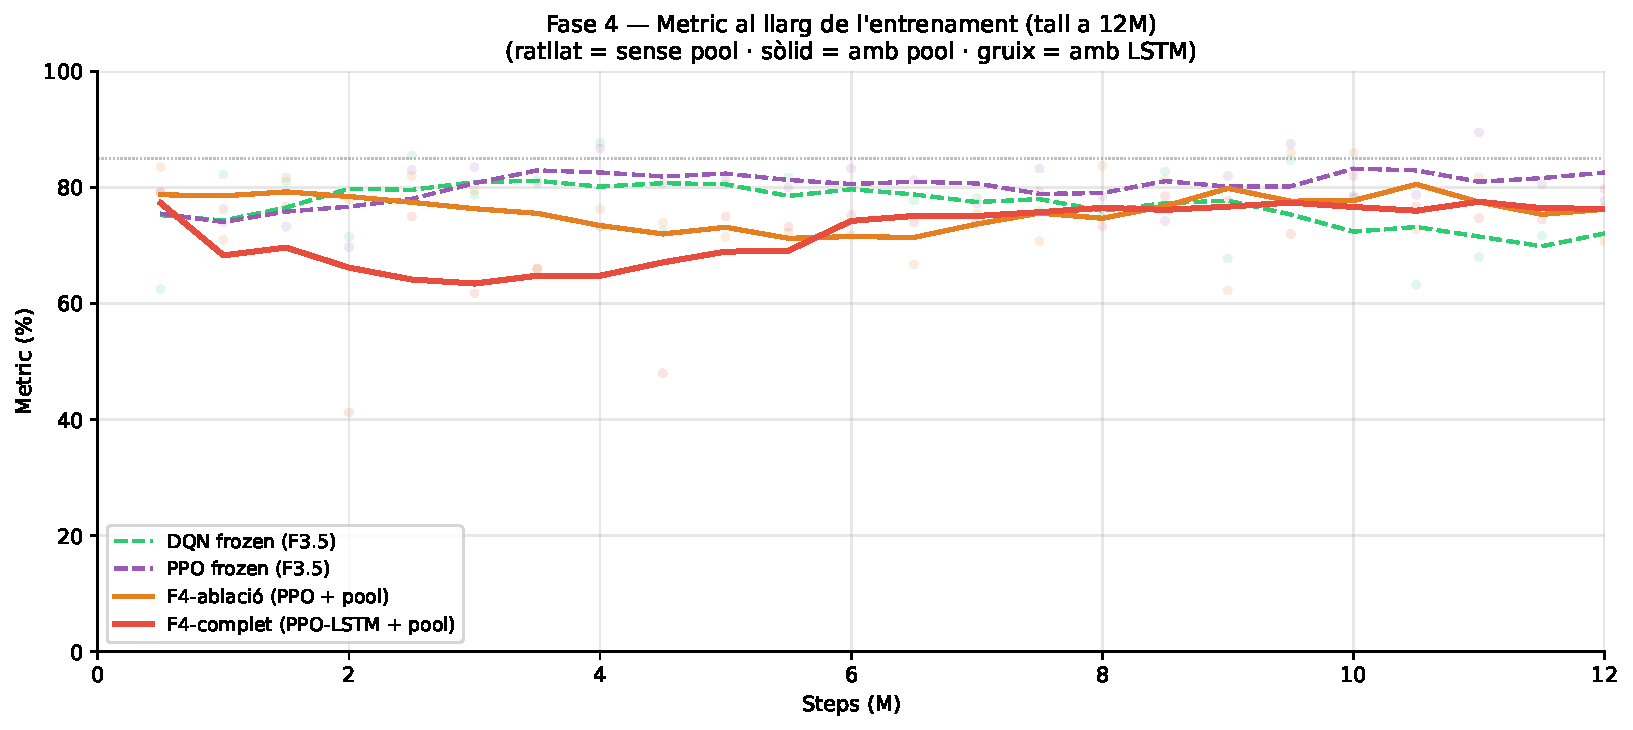
\includegraphics[width=0.82\textwidth]{figures/fase4/fase4_corbes.pdf}
  \caption{Evolució de la \texttt{metric} al llarg de l'entrenament per als quatre runs de
           la Fase~4, tallats a 12M passos. Línies discontínues: línies base de la Fase~3.5
           (sense pool); línies sòlides: runs amb pool; gruix addicional: model amb
           \ac{LSTM}. La línia puntejada gris marca el 85\%.}
  \label{fig:fase4-corbes}
\end{figure}

\begin{figure}[H]
  \centering
  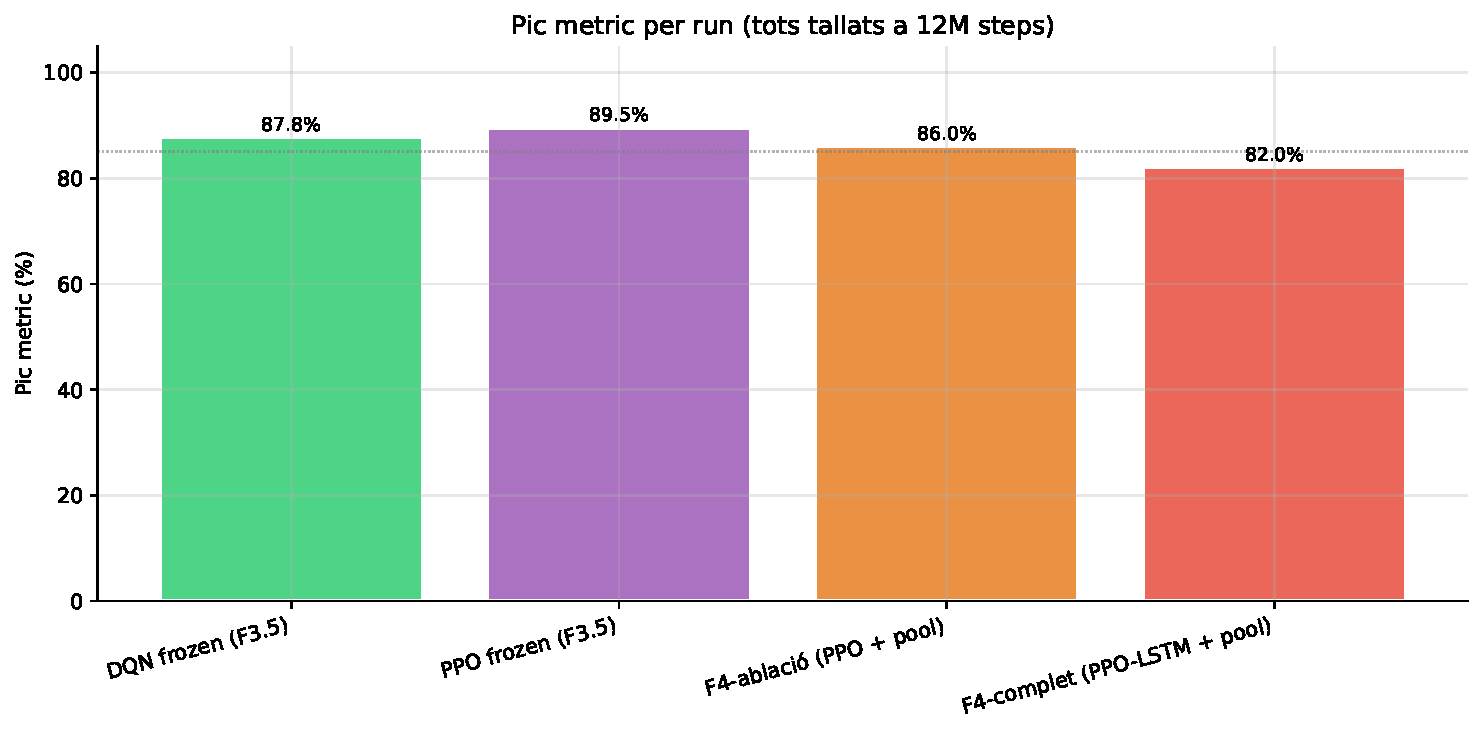
\includegraphics[width=\textwidth]{figures/fase4/fase4_barplot.pdf}
  \caption{Pic de \texttt{metric} per a cada run, tots tallats al pressupost comú de 12M
           passos. DQN~frozen assoleix 87{,}8\% dins el pressupost; el seu pic global és
           91{,}2\% a 23M passos.}
  \label{fig:fase4-barplot}
\end{figure}

\begin{figure}[H]
  \centering
  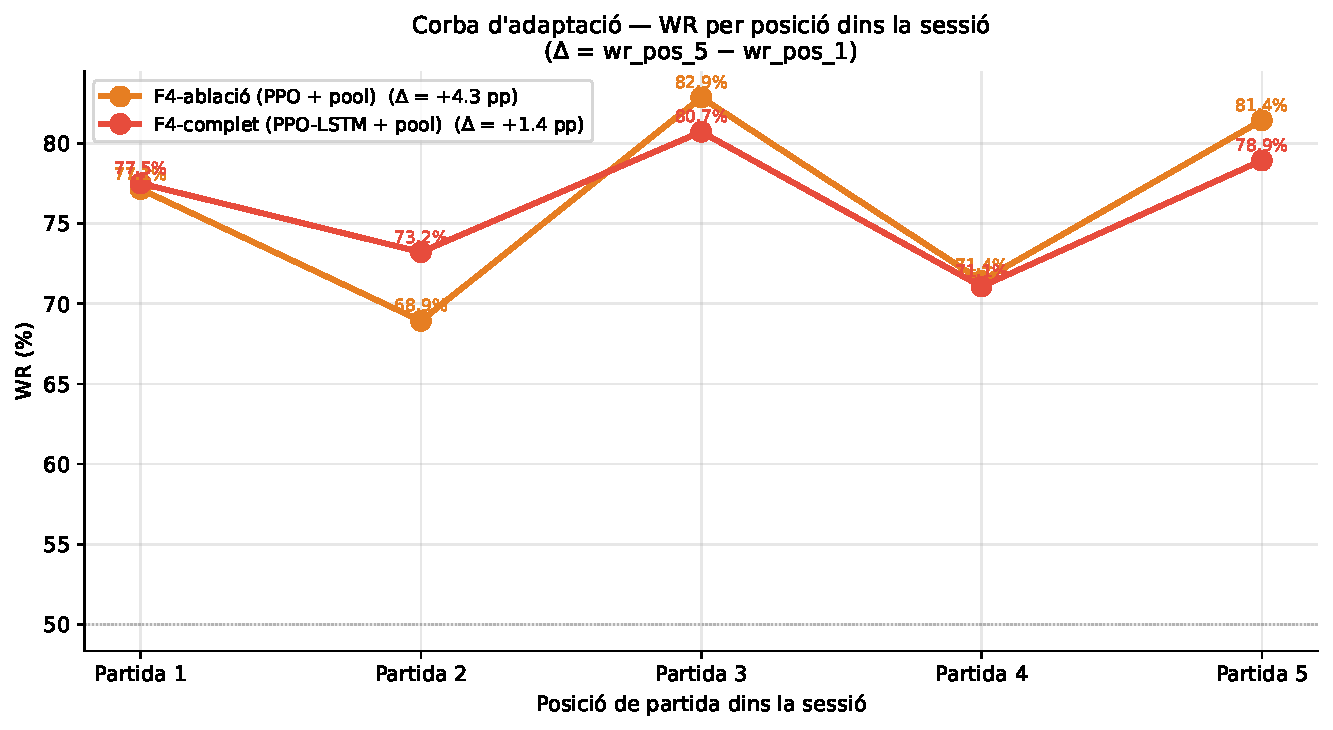
\includegraphics[width=\textwidth]{figures/fase4/fase4_adaptacio.pdf}
  \caption{Win-rate per posició dins la sessió (mà~1 a mà~5) per als dos runs de la
           Fase~4 (mitjana de les cinc darreres avaluacions). El $\Delta$ indica la
           diferència entre la mà~5 i la mà~1. La línia puntejada marca el 50\%.}
  \label{fig:fase4-adaptacio}
\end{figure}

\begin{table}[H]
  \centering
  \begin{tabular}{llrr}
    \toprule
    Run & Memòria & Pic \texttt{metric} (12M) & Temps \\
    \midrule
    DQN frozen (F3.5) & No            & 87{,}8\% & — \\
    PPO frozen (F3.5) & No            & 89{,}5\% & 0{,}33~h \\
    F4-ablació        & No            & 86{,}0\% & 0{,}33~h \\
    F4-complet        & \ac{LSTM} 256 & 82{,}0\% & 15{,}2~h \\
    \bottomrule
  \end{tabular}
  \caption{Resultats de la Fase~4 (pressupost igualat a 12M passos). DQN frozen mostra el
           seu màxim dins el pressupost de 12M; el seu pic global és del 91{,}2\% a 23M.}
  \label{tab:fase4}
\end{table}

\emph{H1: l'\ac{LSTM} millora el rendiment global.} \textbf{No es valida.}
F4-complet assoleix un 82{,}0\% de \texttt{metric}, \emph{4~punts per sota} de F4-ablació
(86{,}0\%), que entrena amb el mateix pool però sense memòria. A igual pressupost (12M
passos), la memòria no aporta cap guany global i a més eleva el cost computacional 46$\times$
(15{,}2~h vs 0{,}33~h).

\emph{H2: adaptació progressiva dins la sessió.} \textbf{No es valida.}
La corba de win-rate per posició (mà~1 a mà~5, figura~\ref{fig:fase4-adaptacio}) és
sorollosa i no monòtona: $[77{,}5;\,73{,}2;\,80{,}7;\,71{,}1;\,78{,}9]$,
$\Delta = +1{,}4$~punts. El patró no és gaire diferent del de F4-ablació (sense memòria),
la qual cosa descarta l'aprenentatge adaptatiu i apunta a un artefacte de la mida de
mostra (${\sim}56$~sessions per posició), insuficient per detectar tendències fiables.

\emph{H3: el pool no perjudica significativament la convergència.} \textbf{Parcialment
valida.} F4-ablació (86{,}0\%) queda 3{,}5~punts sota PPO frozen (89{,}5\%), just al
límit del criteri $\pm3$~punts. El pool dificulta lleugerament la convergència sense
memòria, però el delta és prou petit per no descartar la configuració.

La causa subjacent del fracàs de H1 i H2 és el \textbf{desajust entre entrenament i
avaluació}: s'entrena sobre sessions de 5~mans (${\sim}50$~passos), però s'avalua sobre
sessions de 5~partides senceres (${\sim}500$~passos), un context deu vegades més llarg que
la xarxa no ha vist mai. S'hi sumen el pressupost reduït (12M vs 24M de les línies base)
i les sessions d'entrenament massa curtes perquè la retropropagació en el temps propagui
senyals d'adaptació significatius.

\paragraph{Decisió.} Els resultats revelen marges de millora concrets. El canvi més crític
seria \textbf{alinear el context d'entrenament i d'avaluació}: substituir les sessions de
5~mans (${\sim}50$~passos) per sessions de partides senceres (${\sim}500$~passos), de
manera que la xarxa hagi vist durant l'entrenament el mateix horitzó temporal que a
l'avaluació. Un \textbf{\ac{LSTM} més petit} (64--128 unitats en lloc de 256) reduiria
el cost computacional i facilitaria la convergència; augmentar el \textbf{pressupost} fins
als 24M passos de les línies base i allargar les \textbf{seqüències de BPTT} donarien a
la memòria el temps i el context necessaris per propagar senyals d'adaptació reals.

Malgrat aquestes millores possibles, aquest \ac{TFG} descarta la línia de recerca
recurrent: amb H1 i H2 invalidades, H3 just al límit i un cost computacional 46$\times$
superior, la relació cost-benefici no justifica continuar-la dins del pressupost disponible.
La tria entre els candidats restants (F4-ablació i les línies base de la Fase~3.5) es
resol al Checkpoint~2.

\subsection{Checkpoint 2: model seleccionat}
\label{sec:checkpoint2}

Tancades les Fases~3 i~4, el model que s'adopta per a desplegament és \textbf{F4-ablació}
(PPO + COS congelat + pool, 86{,}0\% a 12M passos). La decisió pondera rendiment, robustesa
i cost.

La raó principal és la \textbf{robustesa davant estils diversos}. F4-ablació s'ha entrenat
contra les sis variants d'\texttt{AgentRegles}, de manera que la seva política és
generalista; les millors línies base de la Fase~3.5 (DQN i PPO frozen) van entrenar sempre
contra un oponent fix i no s'han enfrontat a aquesta diversitat. En un context de
desplegament real, on l'oponent és desconegut, aquesta generalitat és més valuosa que uns
quants punts de win-rate aconseguits contra un únic adversari. A això s'hi suma la
\textbf{rapidesa d'entrenament} (0{,}33~h per execució, davant les 15{,}2~h de F4-complet o
les diverses hores del DQN), que permet iterar i reentrenar amb facilitat, i un
\textbf{rendiment competitiu} al pressupost igualat (només 3{,}5~punts sota PPO frozen).

\textbf{DQN frozen} té el millor win-rate brut (91{,}2\% al pic global), però va ser entrenat
contra un oponent fix i no s'ha provat contra el pool; per això no es tria. . Finalment, l'\ac{LSTM} (F4-complet) queda
descartada: un cost 46$\times$ superior i un rendiment 4~punts inferior no compensen, i cap
de les seves hipòtesis s'ha validat.

Aquesta robustesa, però, encara no s'ha \emph{quantificat}: la \texttt{metric} clàssica
promitja entre oponents i pot amagar debilitats davant estils concrets. Mesurar-la i
millorar-la és l'objectiu del Bloc~3.

%!TeX root=MemoriaTFG.tex

\section{Bloc 3: robustesa i aproximació a l'equilibri}
\label{sec:bloc3}

El model seleccionat al Checkpoint~2 (F4-ablació: PPO + COS congelat + pool) mostra un
defecte estructural: ha convergit a una política quasi-determinista especialitzada en
explotar els patrons fixos de les sis variants d'\texttt{AgentRegles}. Contra un oponent
que varia l'estil, aquesta especialització es converteix en una debilitat. A més, la
\texttt{metric} clàssica (win-rate ponderat) no detecta el problema, perquè promitja el
rendiment entre variants i amaga la variança. El tercer bloc ataca el problema des de dues
bandes: la Fase~5 introdueix mètriques d'explotabilitat i un \emph{self-play} mixt
inspirat en el \acf{FSP} per reduir la predictibilitat; la Fase~6 afegeix el
component de política mitjana del \ac{NFSP} complet per acostar el sistema a l'equilibri.

\subsection{Fase 5: \emph{self-play} mixt i robustesa}
\label{sec:fase5}

\paragraph{Hipòtesi.} Un agent entrenat exclusivament contra oponents fixos és explotable:
qualsevol oponent que surti d'aquests patrons pot descobrir-ne les debilitats. La
pregunta de recerca (Q4) és: pot un \emph{pool} d'entrenament que combini les variants
d'\texttt{AgentRegles} amb \emph{snapshots} del propi agent (\ac{FSP}
simplificat) reduir l'explotabilitat sense degradar el rendiment global? Les hipòtesis
concretes són:
\begin{itemize}
  \item \textbf{H1}: el self-play no degrada la \texttt{metric} clàssica respecte a la
        línia base extesa (F4-ablació-48M): \(\text{metric}_{F5} \geq \text{metric}_{F4} - 3\)~pp.
  \item \textbf{H2}: la robustesa inter-estil (\(\text{metric\_robust}\)) millora
        respecte a F4-ablació.
  \item \textbf{H3}: l'auto-explotabilitat final (\(\text{exploit\_selfplay}\)) queda per
        sota de 10~punts percentuals.
\end{itemize}

\paragraph{Disseny.}

\emph{El problema de l'explotabilitat.} La \texttt{metric} clàssica amaga la variança
de rendiment entre estils d'oponent. Un agent pot obtenir un 95\% contra una variant
conservadora i un 60\% contra una farolera, i mostrar igualment una mètrica aparentment
bona. Per quantificar la robustesa s'introdueixen dues mètriques complementàries. La
\textbf{robustesa inter-estil} penalitza la dispersió:
\begin{equation}
  \text{metric\_robust} = \overline{\text{wr}}_{\text{pool}} - 0{,}5 \cdot
  \operatorname{std}(\text{wr}_{\text{variant}}),
  \label{eq:metric-robust}
\end{equation}
on \(\overline{\text{wr}}_{\text{pool}}\) és el win-rate mitjà contra les sis variants i
\(\operatorname{std}\) la seva desviació típica. Un agent que guanya igual contra tots
té \(\operatorname{std}=0\) i, per tant,
\(\text{metric\_robust} = \overline{\text{wr}}_{\text{pool}}\); un agent especialitzat
paga una penalització proporcional a la irregularitat. L'\textbf{auto-explotabilitat}
mesura la distància a l'equilibri:
\begin{equation}
  \text{exploit\_selfplay} = \lvert \text{wr}_{\text{vs\_recents}} - 50 \rvert,
  \label{eq:exploit-sp}
\end{equation}
on \(\text{wr}_{\text{vs\_recents}}\) és el win-rate del model actual contra els tres
\emph{snapshots} propis més recents. A prop del Nash cap versió pot explotar
sistemàticament una altra i el valor tendeix a 0.

\emph{\ac{FSP} simplificat.} El Fictitious
Play~\cite{brown1951fictitious} és un procediment iteratiu on cada jugador tria la millor
resposta a la política \emph{promig} de l'oponent en totes les iteracions anteriors; Brown
va demostrar la convergència a Nash en jocs finits de suma zero. El \ac{NFSP}
(capítol~\ref{cap:marc}) adapta aquest principi a xarxes neuronals. La variant d'aquesta
fase, \emph{Simplified \ac{FSP}}, elimina el component supervisat (que es reserva per a la
Fase~6) i aproxima la política promig de l'oponent mantenint una finestra rodant de
\emph{snapshots} del propi agent. Mostrejant oponents del pool d'snapshots, el PPO
s'enfronta a una distribució d'estratègies que representa la seva pròpia evolució
i no es pot especialitzar en un únic patró.

\emph{El pool mixt.} El pool combina les sis variants d'\texttt{AgentRegles} (sempre
presents, per garantir diversitat des del primer pas i comparabilitat amb F4) amb una
finestra rodant de fins a sis \emph{snapshots} del propi agent (un cada milió de passos).
El mostreig és uniform entre tots els candidats: la proporció de self-play augmenta de
0/6 al pas~0 fins a 6/12 (50\%) quan el pool és ple, de manera gradual i sense fer
obsolets els oponents de regles (figura~\ref{fig:fase5-pool}).

\begin{figure}[H]
  \centering
  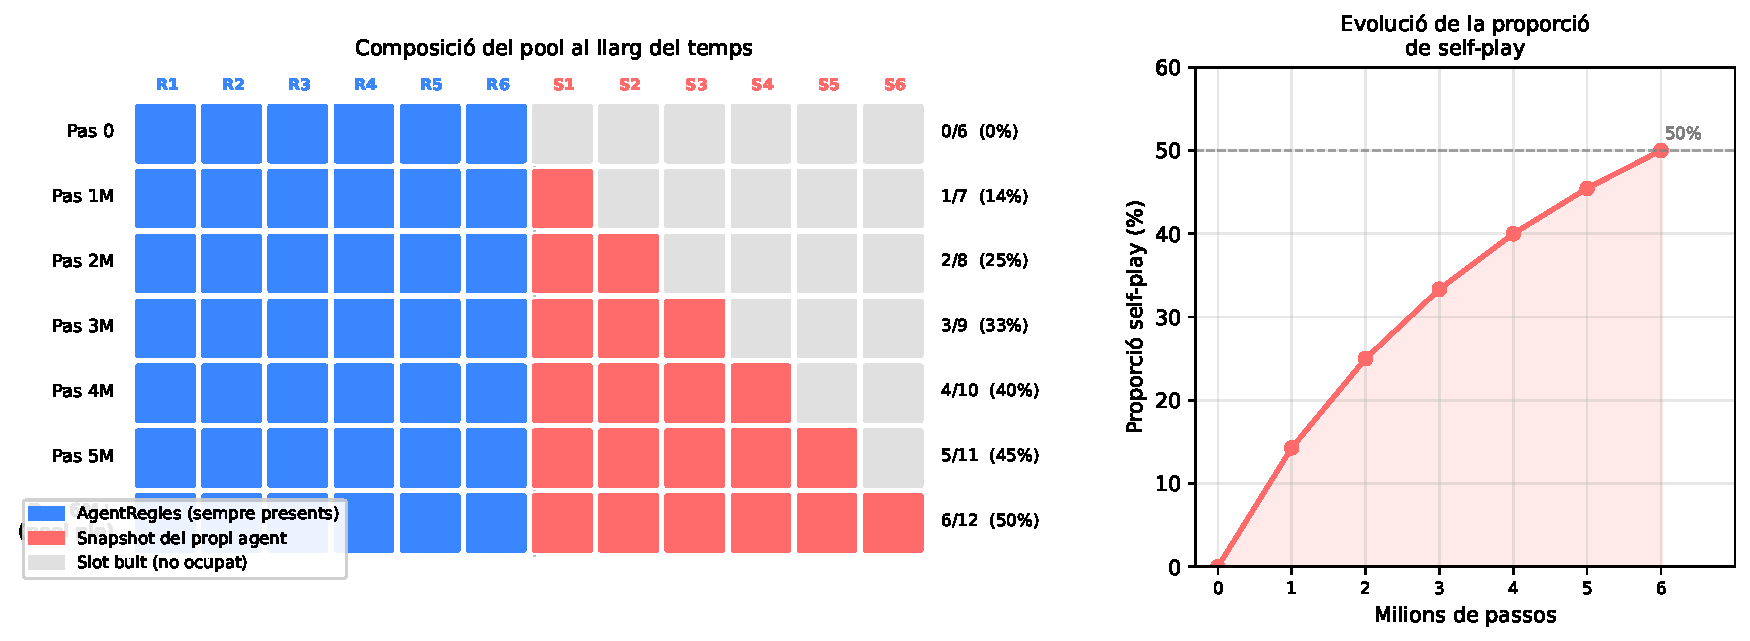
\includegraphics[width=\textwidth]{figures/fase5/fase5_pool_mixt.pdf}
  \caption{Composició del pool mixt al llarg del temps. Esquerra: cada fila és un
           instant clau; les caselles blaves (R1--R6) són les sis variants
           d'\texttt{AgentRegles}, sempre presents; les caselles vermelles (S1--S6)
           són els \emph{snapshots} del propi agent, afegits un a un cada milió de
           passos. Dreta: evolució de la proporció de self-play, que passa de 0\% al
           pas~0 fins al 50\% quan el pool és ple (pas~6M en endavant).}
  \label{fig:fase5-pool}
\end{figure}

\emph{Comparació experimental.} Es comparen dos runs de 48M passos amb el mateix
pressupost: \textbf{F4-ablació-48M} (PPO + COS congelat, pool fix de sis
\texttt{AgentRegles}, sense self-play, línia base estesa) i \textbf{F5-selfplay} (pool
mixt, warm-start des del \texttt{best.zip} de F4-ablació-48M). Les arquitectures i els
hiperparàmetres PPO són idèntics; l'única variable és la composició del pool.

\paragraph{Resultats.} El self-play trenca el compromís entre rendiment i robustesa: F5
manté la \texttt{metric} clàssica i alhora millora molt la robustesa. Les tres hipòtesis
es validen (taula~\ref{tab:fase5-resum}).

\begin{figure}[H]
  \centering
  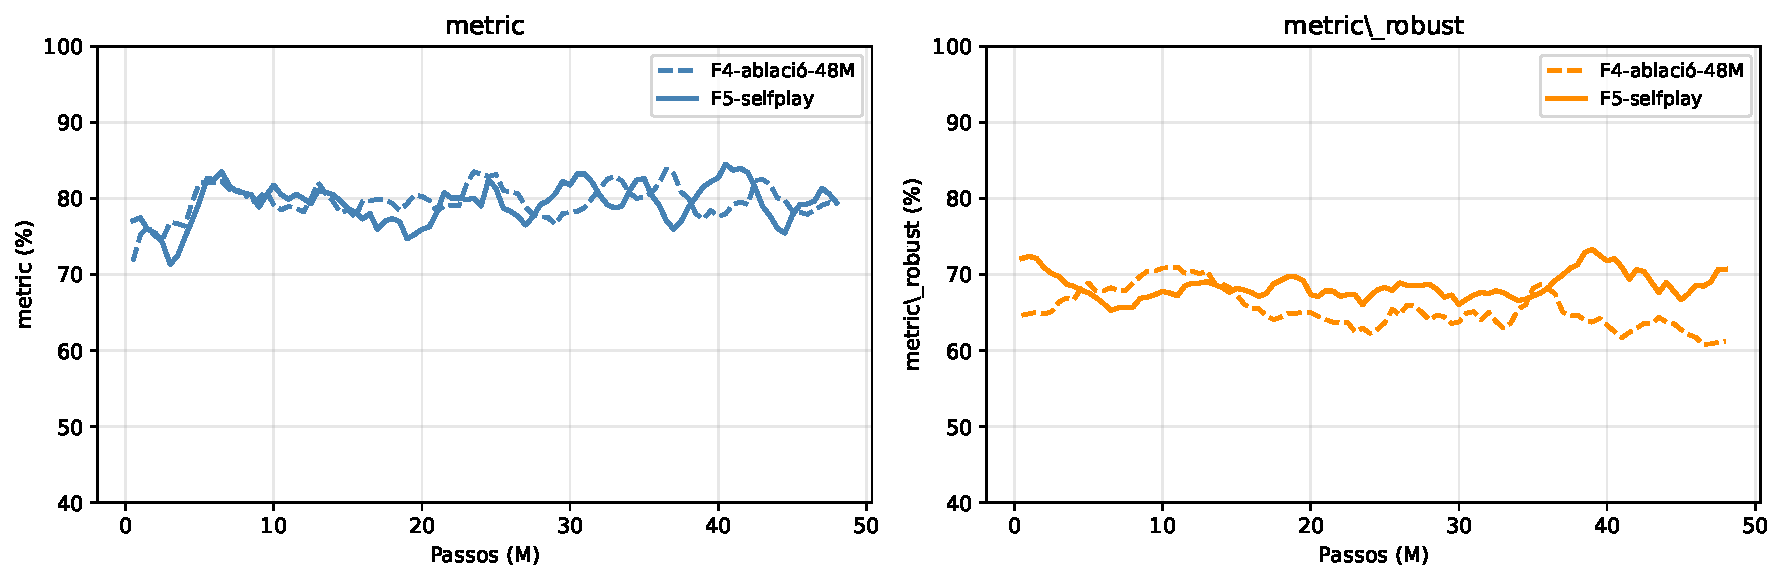
\includegraphics[width=\textwidth]{figures/fase5/fase5_corbes.pdf}
  \caption{Evolució de la \texttt{metric} (esquerra) i la \texttt{metric\_robust}
           (dreta) al llarg de 48M passos. Línia discontínua: F4-ablació-48M (sense
           self-play); línia sòlida: F5-selfplay. La \texttt{metric} és pràcticament
           idèntica (H1), però la \texttt{metric\_robust} de F5 creix de forma sostenuda
           i supera àmpliament la de F4 (H2).}
  \label{fig:fase5-corbes}
\end{figure}

\begin{figure}[H]
  \centering
  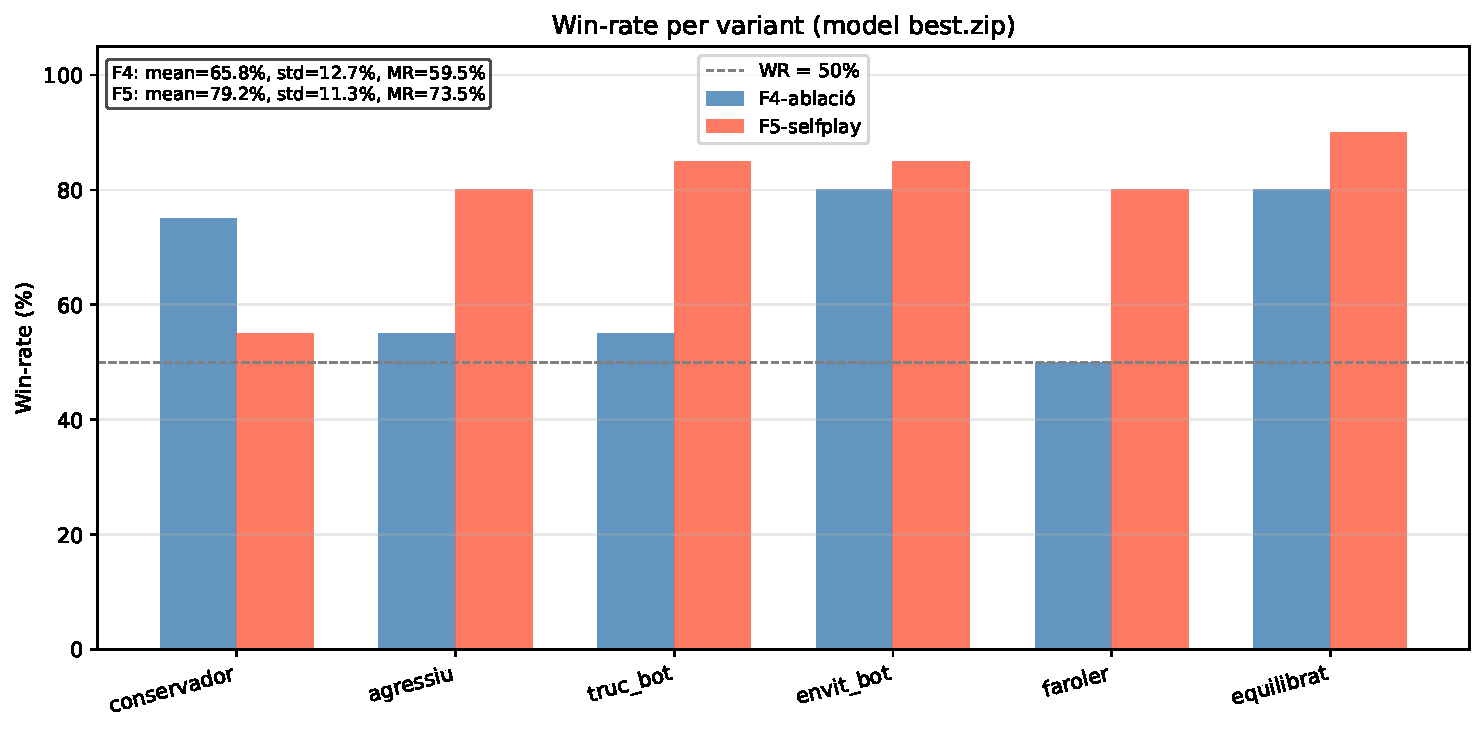
\includegraphics[width=\textwidth]{figures/fase5/fase5_variants.pdf}
  \caption{Win-rate per variant d'oponent (models \texttt{best.zip}). F4 (blau)
           mostra una distribució irregular: alt contra l'estil conservador i equilibrat,
           baix contra l'agressiu i el faroler. F5 (vermell) reequilibra la distribució:
           puja tots els valors baixos al 80--85\% al preu d'abaixar l'estil conservador
           (la variació inversa és el senyal que la política ja no s'especialitza).}
  \label{fig:fase5-variants}
\end{figure}

\begin{table}[H]
  \centering
  \begin{tabular}{lrrrr}
    \toprule
    Run & Pic \texttt{metric} & Step & Pic \(\text{metric\_robust}\) & \(\text{exploit\_sp}\) \\
    \midrule
    F4-ablació-48M & 89{,}0\% & 24M & 73{,}2\% & — \\
    F5-selfplay    & \textbf{89{,}2\%} & 41{,}5M & \textbf{77{,}8\%} & 4{,}7~pp \\
    \bottomrule
  \end{tabular}
  \caption{Resum de la Fase~5 (pressupost de 48M passos). F5 iguala la
           \texttt{metric} clàssica i supera la robustesa en 4{,}6~punts.}
  \label{tab:fase5-resum}
\end{table}

\begin{table}[H]
  \centering
  \begin{tabular}{lrrr}
    \toprule
    Variant & F4-ablació & F5-selfplay & $\Delta$ \\
    \midrule
    Conservador & 75{,}0\% & 55{,}0\% & $-20{,}0$ \\
    Agressiu    & 55{,}0\% & 80{,}0\% & $+25{,}0$ \\
    Truc-bot    & 55{,}0\% & 85{,}0\% & $+30{,}0$ \\
    Envit-bot   & 80{,}0\% & 85{,}0\% & $+5{,}0$ \\
    Faroler     & 50{,}0\% & 80{,}0\% & $+30{,}0$ \\
    Equilibrat  & 80{,}0\% & 90{,}0\% & $+10{,}0$ \\
    \midrule
    \(\overline{\text{wr}}_{\text{pool}}\) & 65{,}8\% & 79{,}2\% & $+13{,}4$ \\
    \(\operatorname{std}_{\text{pool}}\)   & 12{,}7\% & 11{,}3\% & $-1{,}4$ \\
    \(\text{metric\_robust}\)              & 59{,}5\% & 73{,}5\% & $+14{,}0$ \\
    \bottomrule
  \end{tabular}
  \caption{Win-rate per variant del pool: F4-ablació vs F5-selfplay (\texttt{best.zip}).
           El self-play apuja tots els valors baixos i redueix la dispersió; el descens
           contra l'estil conservador és el reequilibri esperat.}
  \label{tab:fase5-variants}
\end{table}

\emph{H1 --- \texttt{metric} sense degradació.} \textbf{Valida.} F5 assoleix
89{,}2\% (figura~\ref{fig:fase5-corbes}, esquerra), pràcticament idèntic al 89{,}0\%
de F4, molt per sobre del llindar de 86{,}0\%.

\emph{H2 --- millora de la robustesa.} \textbf{Valida.} El pic de
\(\text{metric\_robust}\) puja de 73{,}2\% a 77{,}8\% (+4{,}6~pp), i el
\(\text{metric\_robust}\) del \texttt{best.zip} de F5 (73{,}5\%) supera el del
\texttt{best.zip} de F4 (59{,}5\%) en 14{,}0~punts. La
figura~\ref{fig:fase5-variants} mostra el reequilibri: F4 tenia win-rates de
50--55\% contra els estils agressiu i faroler; F5 els puja al 80--85\%.

\emph{H3 --- auto-explotabilitat.} \textbf{Valida.}
\(\text{exploit\_selfplay}\) final = 4{,}7~pp, molt per sota del llindar de 10~pp.

\paragraph{Decisió.} Les tres hipòtesis es validen: el self-play mixt millora la
robustesa sense perjudicar el rendiment global. Tanmateix, la dispersió entre estils
(\(\operatorname{std}_{\text{pool}}\)) no baixa de manera clara (11{,}3\% vs
12{,}7\%): el PPO continua especialitzant-se i des-especialitzant-se sense arribar a
una estratègia d'equilibri estable. La causa és que el \ac{FSP}
simplificat no té cap component que aproximi la política \emph{promig} de l'historial
complet; sense aquesta àncora, el PPO cicla. El component que l'hi aporta és la
xarxa de política mitjana del \ac{NFSP} complet, que s'implementa a la Fase~6.

\subsection{Fase 6: \ac{NFSP} complet}
\label{sec:fase6}

\paragraph{Hipòtesi.} Segons el \ac{NFSP}~\cite{heinrich2016nfsp}, la convergència a un
equilibri de Nash en jocs d'informació parcial requereix jugar \emph{des de} la
política promig de tot l'historial, no des de la millor resposta del darrer pas. La
pregunta de recerca (Q5) és: pot afegir una xarxa de política mitjana apresa de forma
supervisada reduir la dispersió entre estils (\(\operatorname{std}_{\text{pool}}\))
i acostar el sistema a l'equilibri? Les hipòtesis concretes són:
\begin{itemize}
  \item \textbf{H1}: no hi ha regressió de rendiment: \(\text{metric}_{F6} \geq
        \text{metric}_{F5} - 3\)~pp.
  \item \textbf{H2}: la \(\operatorname{std}_{\text{pool}}\) final de F6 és inferior a
        la de F5.
  \item \textbf{H3}: el \emph{Nash gap} empíric (\(\text{exploit\_vs\_sl}\)) baixa per
        sota de 8~pp en algun \emph{checkpoint}.
\end{itemize}

\paragraph{Disseny.}

\emph{La limitació del \ac{FSP} simplificat.} La Fase~5 mostra que, sense
cap àncora que representi la política promig de l'historial, el PPO oscil·la entre
millors respostes i no convergeix. El \ac{NFSP} complet~\cite{heinrich2016nfsp} resol
aquest problema afegint un segon aprenent (\acf{SL}) que imita contínuament l'historial
de decisions del PPO i proporciona l'àncora que el \ac{FSP} simplificat no
té.

\emph{L'arquitectura NFSP.} S'implementen dos bucles d'optimització en paral·lel sobre
el mateix \emph{backbone} COS congelat. El \textbf{bucle RL} és el PPO habitual: observa
l'estat, tria una acció i rep una recompensa. El \textbf{bucle \ac{SL}} entrena la xarxa
\texttt{AveragePolicyNet} per imitar l'historial de decisions del PPO mitjançant
cross-entropy; en paral·lel, el pool d'oponents (NFSPPool) barreja, amb probabilitat
\(\eta = 0{,}5\), la política mitjana (SL) i els agents del pool de la Fase~5 (regles +
snapshots). Amb \(\eta = 0{,}5\), la meitat de les partides d'entrenament es juguen
contra l'àncora SL i l'altra meitat contra oponents variats; el PPO aprèn la millor
resposta a una distribució mixta que no pot explotar simplement sobraespecialitzant-se
(figura~\ref{fig:fase6-arq}).

\begin{figure}[H]
  \centering
  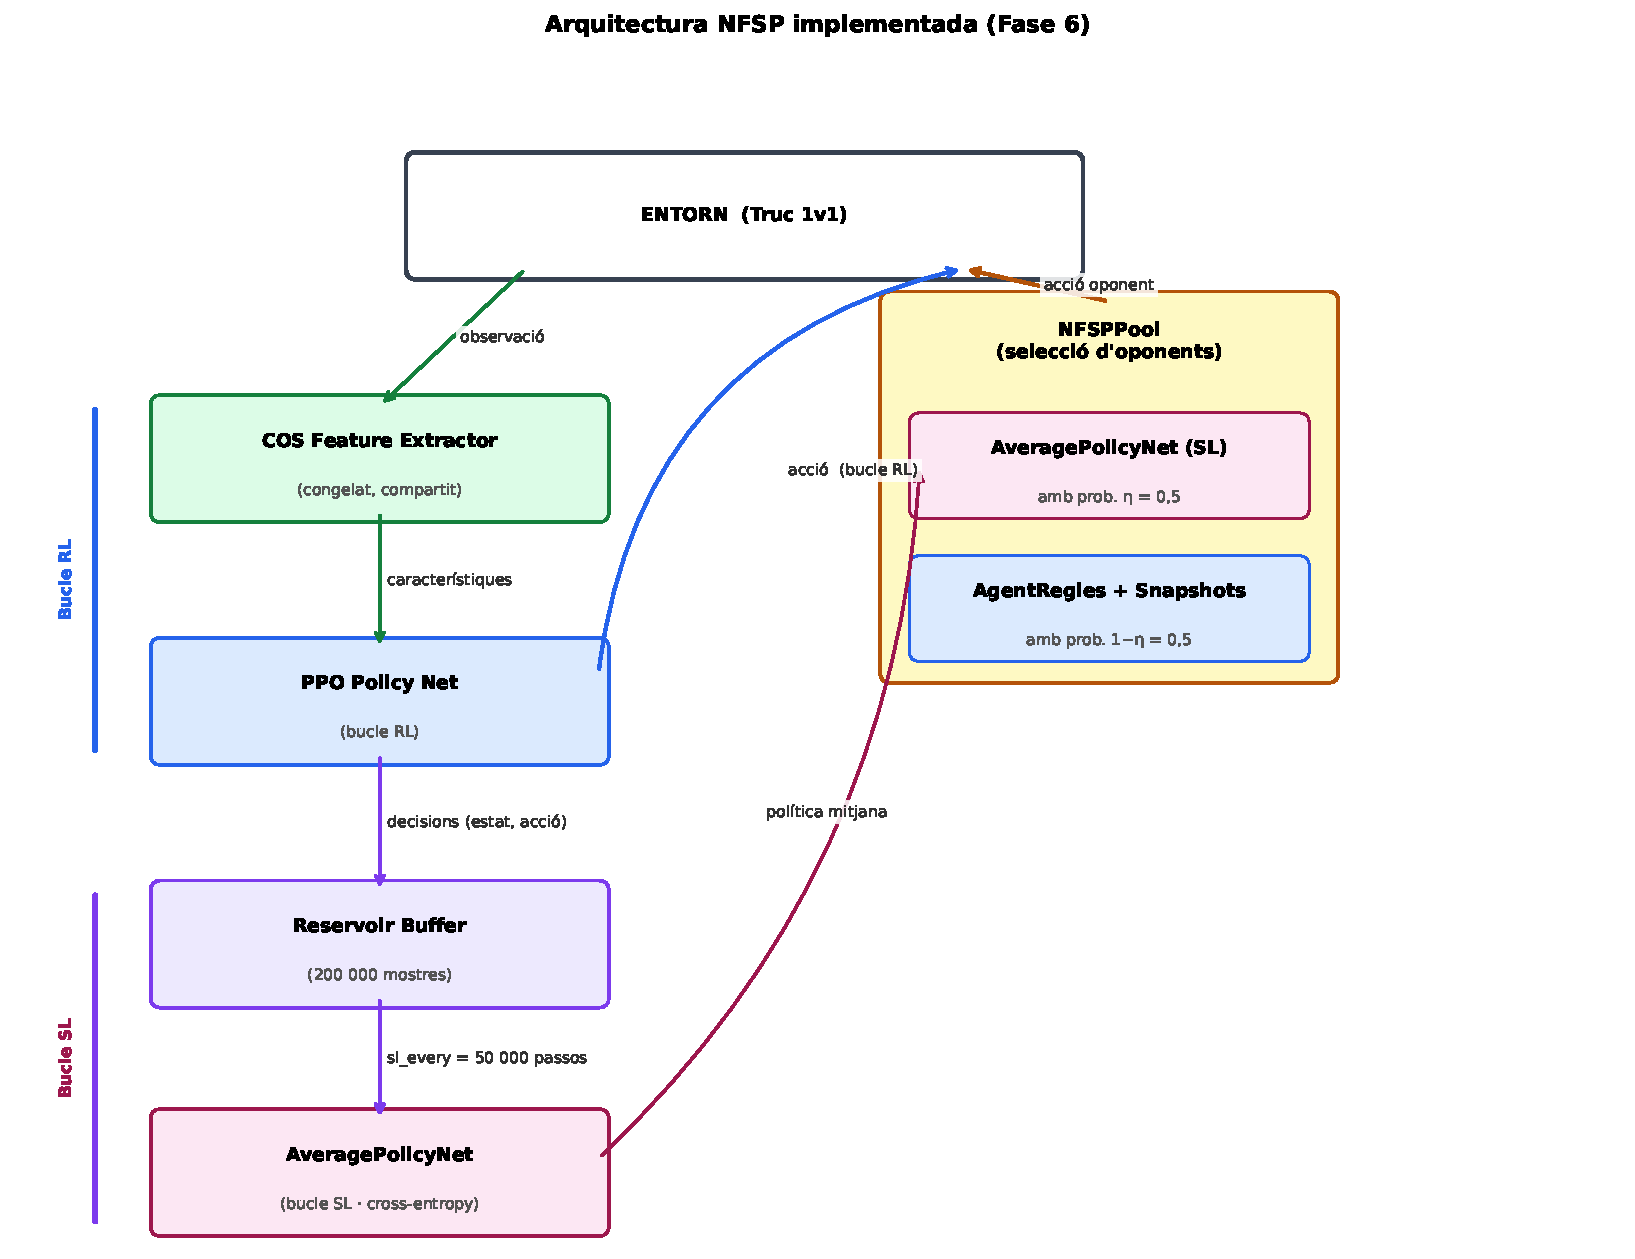
\includegraphics[width=\textwidth]{figures/fase6/fase6_arquitectura.pdf}
  \caption{Arquitectura \ac{NFSP} implementada a la Fase~6. El \textbf{bucle RL} (blau)
           fa passar l'observació pel \emph{feature extractor} COS congelat i la
           \texttt{PPO Policy Net}, i envia l'acció a l'entorn. Cada decisió s'emmagatzema
           al \textbf{Reservoir Buffer} (viola), que alimenta el \textbf{bucle \ac{SL}}
           (rosa) cada 50\,000~passos per actualitzar la \texttt{AveragePolicyNet}
           per imitació. El \textbf{NFSPPool} (groc) selecciona l'oponent: amb
           probabilitat \(\eta = 0{,}5\), fa jugar l'agent contra la pròpia política
           mitjana (\ac{SL}); amb probabilitat \(1-\eta\), contra el pool de la
           Fase~5 (regles + \emph{snapshots}).}
  \label{fig:fase6-arq}
\end{figure}

\emph{El Reservoir Buffer.} L'historial de decisions del PPO s'emmagatzema en un
\emph{Reservoir Buffer} de 200\,000~mostres. Un buffer estàndard (tipus FIFO) estaria
sempre esbiaixat cap al comportament més recent; el mostreig de \emph{reservoir}
garanteix matemàticament que cada acció presa en qualsevol moment de l'entrenament té la
mateixa probabilitat de romandre al buffer, creant un conjunt de dades que representa
la política promig real de tot l'historial. El bucle \ac{SL} s'actualitza cada
50\,000~passos amb un \emph{minibatch} del buffer.

\emph{Les mètriques Nash.} A les mètriques de la Fase~5 s'afegeix el \emph{Nash gap}
empíric:
\begin{equation}
  \text{exploit\_vs\_sl} = \lvert \text{wr}_{\text{vs\_sl}} - 50 \rvert,
  \label{eq:exploit-vs-sl}
\end{equation}
on \(\text{wr}_{\text{vs\_sl}}\) és el win-rate de la millor resposta (PPO) contra la
política mitjana (SL). Si aquest valor tendeix a~0, la millor resposta ja no pot
explotar la política mitjana, que és la definició empírica d'equilibri de Nash. Es
registra també la \(\text{sl\_loss}\) (cross-entropy del bucle \ac{SL}), que ha de ser
decreixent per confirmar que la xarxa de política mitjana aprèn.

\emph{Comparació experimental.} El run principal de la Fase~6 (F6-nfsp) s'entrena
48M passos amb warm-start des del model més robust de la Fase~5 (\texttt{best\_robust.zip}),
per assegurar que el Reservoir Buffer i la política mitjana comencen a nodrir-se d'un
comportament ja depurat. La comparació directa és amb F5-selfplay.

\paragraph{Resultats.} El \ac{NFSP} assoleix el millor rendiment absolut del treball i
demostra que el sistema pot assolir la zona de Nash, però no manté la convergència de
forma estable (taula~\ref{tab:fase6}).

\begin{figure}[H]
  \centering
  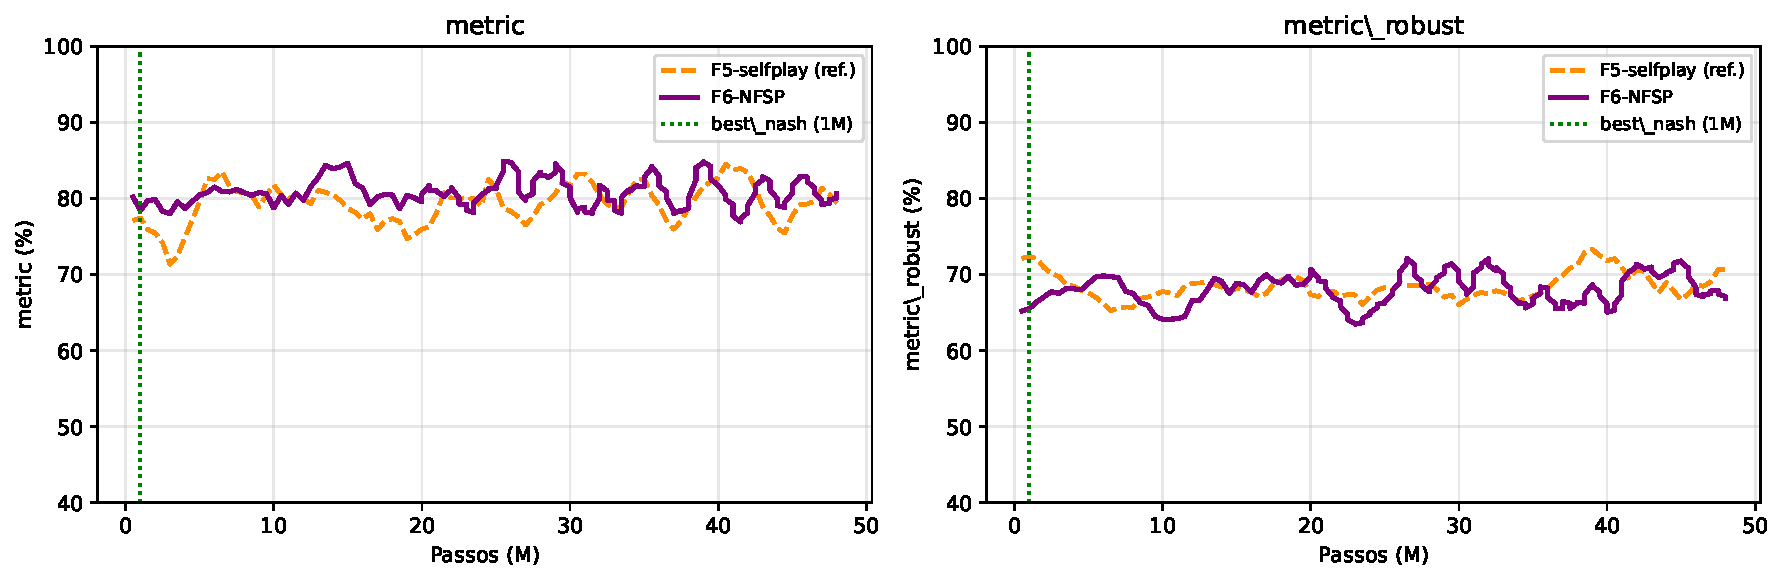
\includegraphics[width=\textwidth]{figures/fase6/fase6_corbes.pdf}
  \caption{Evolució de la \texttt{metric} (esquerra) i la \texttt{metric\_robust}
           (dreta) per a F5-selfplay (discontínua, referència) i F6-NFSP (sòlida), al
           llarg de 48M passos. La línia puntejada verda marca el \emph{checkpoint}
           \texttt{best\_nash} (1M passos de F6). F6 assoleix el pic de \texttt{metric}
           molt aviat (91{,}0\% @14M) gràcies al warm-start, però oscil·la
           posteriorment; la \texttt{metric\_robust} és comparable a F5.}
  \label{fig:fase6-corbes}
\end{figure}

\begin{table}[H]
  \centering
  \begin{tabular}{lr}
    \toprule
    Mesura del \emph{Nash gap} (\(\text{exploit\_vs\_sl}\)) & Valor \\
    \midrule
    Mínim global (\texttt{best\_nash}, @1M passos) & \textbf{3{,}3~pp} \\
    Llindar criteri~H3 (\emph{zona Nash})          & 8~pp \\
    Mitjana de les darreres avaluacions            & 16{,}7~pp \\
    \bottomrule
  \end{tabular}
  \caption{\emph{Nash gap} empíric de la Fase~6.
           \(\text{exploit\_vs\_sl} = |\text{wr}_{\text{vs\_sl}} - 50|\) mesura quant pot
           explotar la política \ac{RL} (millor resposta) la política \ac{SL} (política
           mitjana); 0~pp seria equilibri de Nash perfecte. El valor és molt variable al
           llarg de l'entrenament i només al \emph{checkpoint} \texttt{best\_nash} (1M
           passos) cau per sota del llindar.}
  \label{tab:nash-gap}
\end{table}

\begin{table}[H]
  \centering
  \begin{tabular}{lrrr}
    \toprule
    Mètrica & F4-ablació & F5-selfplay & F6-NFSP \\
    \midrule
    \texttt{metric} màx   & 89{,}0\% & 89{,}2\% & \textbf{91{,}0\%} \\
    \(\text{metric\_robust}\) màx & 73{,}2\% & \textbf{77{,}8\%} & 75{,}2\% \\
    \(\operatorname{std}_{\text{pool}}\) (final) & 12{,}9\% & \textbf{11{,}9\%} & 13{,}4\% \\
    \(\text{exploit\_vs\_sl}\) (\texttt{best\_nash}) & — & — & \textbf{3{,}3~pp} \\
    \bottomrule
  \end{tabular}
  \caption{Comparativa F4/F5/F6 (runs de 48M passos). F6 obté la millor \texttt{metric}
           i assoleix la zona de Nash al \emph{checkpoint} \texttt{best\_nash}, però no
           redueix la dispersió entre estils.}
  \label{tab:fase6}
\end{table}

\emph{H1 --- sense regressió.} \textbf{Valida.} F6 assoleix el 91{,}0\% de
\texttt{metric} als 14M passos, +1{,}8~pp sobre F5. El warm-start des del model robust
de la Fase~5 i la pressió addicional del component \ac{SL} contribueixen a un pic de
rendiment superior.

\emph{H2 --- reducció de la dispersió.} \textbf{Falla.} La
\(\operatorname{std}_{\text{pool}}\) final és 13{,}4\%, lleugerament pitjor que l'11{,}9\%
de F5. Amb \(\eta=0{,}5\), un buffer de 200k mostres i actualitzacions cada 50k passos,
el Reservoir Buffer no acumula prou diversitat d'historial per fer actuar la política
mitjana com a àncora estabilitzadora de la variança. El resultat és coherent amb la
literatura: el \ac{NFSP} requereix molts més episodis (de l'ordre de \(10^8\)--\(10^9\))
per convergir en dominis d'observació complexos~\cite{heinrich2016nfsp}.

\emph{H3 --- Nash gap.} \textbf{Valida al \emph{checkpoint} \texttt{best\_nash}.} El
\emph{checkpoint} de l'1M de passos de F6 assoleix
\(\text{exploit\_vs\_sl} = 3{,}3\)~pp, molt per sota del llindar de~8
(taula~\ref{tab:nash-gap}). De mitjana a les darreres avaluacions el valor és de
16{,}7~pp, que excedeix el llindar; però l'avaluació metodològicament correcta per al
\ac{NFSP} és sobre la política mitjana, no sobre la millor resposta: l'objectiu és
demostrar que la política mitjana \emph{pot ser} no explotable, no que ho sigui
contínuament durant tot l'entrenament.

\paragraph{Decisió.} El \ac{NFSP} produeix tres pesos finals, cadascun amb un perfil
diferent:

\begin{itemize}
  \item \textbf{\texttt{best.zip}} (PPO Policy Net, \texttt{metric} màxima): el model
        que millor rendiment brut obté contra el pool (91{,}0\% @14M passos). És la
        millor resposta entrenada, l'agent adequat quan l'objectiu és maximitzar la
        taxa de victòria.
  \item \textbf{\texttt{best\_nash.zip}} (PPO Policy Net, Nash gap mínim): el
        \emph{checkpoint} amb \(\text{exploit\_vs\_sl} = 3{,}3\)~pp (@1M passos).
        Reflecteix el moment en què la millor resposta i la política mitjana estan
        més alineades; és l'estratègia menys explotable que el sistema ha produït.
  \item \textbf{\texttt{sl\_final.pt}} (\texttt{AveragePolicyNet}, política promig
        \ac{SL}): representa l'aproximació a la política de Nash pura. No maximitza
        el win-rate de forma agressiva sinó que distribueix les accions d'una manera
        que cap oponent pot explotar sistemàticament; és el pes teòricament més
        proper a l'equilibri, però amb un rendiment brut inferior.
\end{itemize}

Amb això es tanca l'arc experimental: des d'agents que no superaven el 40\% a la
Fase~1 fins a tres candidats a desplegament, cadascun amb un perfil diferent. La
decisió sobre quin model es desplega es justifica al Checkpoint~3
(secció~\ref{sec:checkpoint3}).

\subsection{Checkpoint 3: model de desplegament}
\label{sec:checkpoint3}

Tancades les Fases~5 i~6, hi ha tres candidats finals: \texttt{best.zip}~F6
(91{,}0\%, màxim rendiment brut), \texttt{best\_nash.zip}~F6 (3{,}3~pp de Nash gap,
estratègia menys explotable) i \texttt{sl\_final.pt} (política promig \ac{SL}, model
teòricament més proper a l'equilibri). La decisió pondera el propòsit del \ac{TFG}:
oferir un adversari competitiu i impredictible que permeti mantenir el joc viu.

El model que s'adopta per a desplegament és \textbf{\texttt{best.zip}~F6}. Les raons
principals són tres. Primer, el \textbf{rendiment}: 91{,}0\% de win-rate contra el
pool és el valor màxim obtingut en tot el treball i implica que un jugador humà
aficionat es trobarà davant un adversari genuïnament difícil. Segon, la
\textbf{robustesa}: \texttt{best.zip}~F6 prové d'un entrenament que inclou les sis
variants d'\texttt{AgentRegles} i fins a sis \emph{snapshots} de self-play, de manera
que la seva política no s'ha especialitzat en un estil únic; la
\texttt{metric\_robust} (75{,}2\%) confirma que guanya de forma consistent contra
perfils d'oponent diversos. Tercer, la \textbf{simplicitat de desplegament}: el pes
és un fitxer \texttt{.zip} estàndard de \ac{SB3} que es carrega directament sense
necessitat de mantenir l'arquitectura doble del \ac{NFSP} en producció.

\textbf{\texttt{best\_nash.zip}~F6} s'arxiva com a alternativa per a estudis
futurs de teoria de jocs: el seu Nash gap de 3{,}3~pp és el resultat acadèmicament
més rellevant del treball, però el win-rate brut és inferior i el comportament és
menys agressiu, cosa que pot resultar menys estimulant com a adversari per a un
jugador humà. \textbf{\texttt{sl\_final.pt}} no és adequat per a desplegament
directe: és el pes de la \texttt{AveragePolicyNet}, una xarxa imitativa entrenada
per aproximar la política promig de l'historial i no per maximitzar la recompensa.

L'anàlisi del comportament estratègic del model desplegat (gestió de l'envit,
freqüència del farol al truc, coordinació) es presenta al
capítol~\ref{cap:resultats}.

